% ======================================================================
% FINAL SUBMISSION MASTER
% Target journal: Applied Intelligence
% Manuscript: Can Sparse Floating Car Data Reliably Forecast Highway Speeds?
%             A Multi-Horizon Evaluation of Forecasting Models
% ======================================================================
% Compiler: pdfLaTeX
% Class: Springer Nature sn-jnl
% Style: sn-basic, numbered citations
% Bibliography database: references.bib
% Keep this TEX file, references.bib, sn-jnl.cls, and Fig1.png--Fig6.png
% in the same project root when compiling.
% ======================================================================

\documentclass[pdflatex,sn-basic,Numbered]{sn-jnl}

% ======================================================================
% PACKAGES
% ======================================================================

\usepackage{graphicx}
\usepackage{amsmath,amssymb,amsfonts}
\usepackage{mathrsfs}
\usepackage{booktabs}
\usepackage{multirow}
\usepackage{array}
\usepackage{tabularx}
\usepackage{xcolor}
\usepackage{textcomp}
\usepackage{xurl}
\usepackage{placeins}

\setlength{\emergencystretch}{2em}
\setlength{\textfloatsep}{7pt plus 2pt minus 1pt}
\setlength{\floatsep}{6pt plus 2pt minus 1pt}
\setlength{\intextsep}{7pt plus 2pt minus 1pt}
\setlength{\tabcolsep}{4pt}
\renewcommand{\arraystretch}{1.06}
\setlength{\arrayrulewidth}{0.45pt}
\setlength{\abovecaptionskip}{4pt}
\setlength{\belowcaptionskip}{2pt}
\widowpenalty=10000
\clubpenalty=10000
\displaywidowpenalty=10000

% Compact explanatory note placed directly beneath each figure caption.
\newcommand{\figurenote}[1]{%
  \par\vspace{1pt}\noindent{\footnotesize\itshape Note: }%
  {\footnotesize #1}\par\vspace{1pt}%
}

\begin{document}

% ======================================================================
% TITLE
% ======================================================================

\title[Multi-Horizon Highway Speed Forecasting from Sparse FCD]
{Can Sparse Floating Car Data Reliably Forecast Highway Speeds? A Multi-Horizon Evaluation of Forecasting Models}

% ======================================================================
% AUTHORS
% ======================================================================

\author*[1]{\fnm{Wenjie} \sur{Sun}}
\email{sunwenjie@graduate.utm.my}

\author*[1]{\fnm{Safizahanin binti} \sur{Mokhtar}}
\email{safizahanin@utm.my}

\author[1]{\fnm{Gabriel} \sur{Ling Hoh Teck}}
\email{gabriel.ling@utm.my}

\author[2]{\fnm{Ruiqing} \sur{Li}}
\email{liruiqing@graduate.utm.my}

\author[3]{\fnm{Lvmin} \sur{Liu}}
\email{llm1194568495@gmail.com}

% ======================================================================
% AFFILIATIONS
% ======================================================================

\affil*[1]{%
  \orgdiv{Department of Urban and Regional Planning},
  \orgname{Universiti Teknologi Malaysia},
  \orgaddress{%
    \city{Skudai},
    \postcode{81310},
    \state{Johor},
    \country{Malaysia}
  }
}

\affil[2]{%
  \orgdiv{Faculty of Computing},
  \orgname{Universiti Teknologi Malaysia},
  \orgaddress{%
    \city{Johor Bahru},
    \postcode{81310},
    \state{Johor},
    \country{Malaysia}
  }
}

\affil[3]{%
  \orgdiv{School of Information Engineering},
  \orgname{Nanjing Normal University Taizhou College},
  \orgaddress{%
    \city{Taizhou},
    \state{Jiangsu Province},
    \country{China}
  }
}

% ======================================================================
% ABSTRACT
% ======================================================================
% Compact problem--method--evidence--boundary structure; numerical claims
% are identical to the frozen formal results reported in the main text.
% ======================================================================

\abstract{%
Evaluating highway speed forecasts is challenging where fixed roadside sensing is sparse and commercial floating car data (FCD) are incomplete.
When FCD are obtained through an application programming interface (API), planned observations may be omitted rather than returned as explicit missing values, while model comparisons can be biased by unequal evaluation samples or temporally non-causal preprocessing.
We address these issues with the Grid-Reconstructed, Auditable, Temporally Causal, and Eligibility-Gated Multi-Horizon FCD Forecasting (GATE-FCD) framework.
GATE-FCD reconstructs the planned observation grid, applies explicit eligibility rules, freezes common sample manifests, and restricts preprocessing to information available before each forecast origin.
Historical Average, Seasonal Historical Average (SeasonalHA), Persistence, Ridge, XGBoost, and a Gated Recurrent Unit (GRU) are evaluated at 51 virtual nodes using 24-h histories, six retrospective rolling-origin folds, and 1-, 3-, and 6-h future-window targets (H1, H3, and H6).
XGBoost achieved the lowest descriptive mean absolute error (MAE) at H1, H3, and H6 (0.949, 0.829, and 0.752~km~h$^{-1}$, respectively), although SeasonalHA remained competitive and fold-level inference did not establish a stable advantage.
These findings highlight the importance of auditable sample construction and temporally causal evaluation when benchmarking forecasting models with incomplete commercial FCD.
}

% ======================================================================
% KEYWORDS
% ======================================================================

\keywords{
floating car data,
traffic speed forecasting,
multi-horizon forecasting,
model reliability,
rolling-origin evaluation,
intelligent transportation systems
}

\maketitle

% ======================================================================
% 1 INTRODUCTION
% ======================================================================

\section{Introduction}
\label{sec:introduction}

Reliable speed forecasts support traffic management, route guidance, and other intelligent transportation system functions. Long-distance highways present a particular sensing problem because continuous roadside detection is expensive to deploy and maintain over large spatial extents. Floating car data (FCD) offer a practical alternative by providing speed and travel-time information without a dense network of fixed detectors. Recent work has used FCD for speed estimation, congestion analysis, traffic-state monitoring, and forecasting \cite{Zhang2025FCD}. Commercial FCD have also been combined with lower-cost sensing sources where conventional monitoring is limited \cite{Ipekyuz2025FCD}. The remaining question for forecasting is not simply whether FCD are available, but whether the observations returned by a commercial service can be converted into a consistent and auditable time series.

Commercial FCD differ from conventional detector data in several ways that matter for evaluation. Services such as TomTom provide provider-processed speed and travel-time estimates through an application programming interface (API) rather than raw vehicle trajectories, leaving upstream sampling, map matching, aggregation, and filtering outside the user's control. More importantly, a planned node--time observation may be absent from the API response altogether rather than appearing as an explicit null. The Pan Borneo Highway dataset used here illustrates this problem: 51 fixed virtual nodes cover an approximately 130-km corridor, but observations are spatially discrete and their temporal coverage, confidence, and gap lengths vary by node and time. If returned rows are treated as a complete series, unreturned observations disappear from the denominator and the distinction among missing, quality-ineligible, and imputed values becomes unclear. That ambiguity can change which forecast origins are available to each model.

Prior research addresses the main components of this problem, but usually in separate workflows. Commercial and vehicle-level FCD have been used for traffic-state estimation and prediction \cite{Ipekyuz2025FCD,Yu2024AutoformerFCD}. Multi-horizon studies have compared naive, statistical, machine-learning, and deep-learning models and have shown that relative performance can change with forecast horizon \cite{Hadry2025TrafficForecasting,Zeb2024FeatureProjection}. A separate body of work treats incomplete traffic observations through completion, imputation, or joint prediction--imputation methods \cite{Chen2024TrafficCompletion,Bikram2024Imputation,Qu2024TrafficPredictionImputation,Zhang2024MissingData}. These strands provide the necessary methods, but they do not by themselves ensure that sparse API-derived FCD are evaluated on a fixed observation space, with the same forecast cases and the same temporal information boundaries across models.

Applying these methods to sparse commercial FCD exposes three evaluation problems. Planned node--time combinations must first be reconstructed before completeness and eligibility can be measured. Model comparisons can otherwise be confounded if different predictors retain different origins or use different missing-value treatments. Temporal order also has to be enforced inside preprocessing: a chronological train--test split does not prevent leakage if normalization, imputation, or feature statistics use information unavailable at the forecast origin \cite{Hewamalage2023ForecastEvaluation}. Finally, one test interval and one mean error cannot show whether a small model advantage persists across time, locations, forecast horizons, or history-reliability conditions. When differences between simple and complex models are small, stability under common causal samples is more informative than the mean ranking alone.

The analysis addresses three questions: (i) can sparse API-derived FCD support 1-, 3-, and 6-h future-window mean-speed forecasting after explicit observation and target eligibility checks; (ii) how do Historical Average (HA), Seasonal Historical Average (SeasonalHA), Persistence, Ridge, XGBoost, and Gated Recurrent Unit (GRU) compare when they use identical forecast origins and target definitions; and (iii) how stable are those comparisons across rolling-origin folds, random seeds, and history-reliability conditions? We address these questions with the Grid-Reconstructed, Auditable, Temporally Causal, and Eligibility-Gated Multi-Horizon FCD Forecasting framework (GATE-FCD). GATE-FCD reconstructs the planned node--time grid, distinguishes missing and quality-ineligible observations, creates a causal 24-h history, and freezes a common sample manifest before model fitting. Six models are then evaluated across six retrospective rolling-origin folds and three horizons. This design isolates differences in forecasting behavior from differences in sample composition and makes it possible to examine where a small accuracy gain is stable and where it reverses.

Section~\ref{sec:related} reviews FCD forecasting, model complexity, and incomplete-data evaluation. Section~\ref{sec:dataset} defines the corridor, reconstructed observation grid, eligibility rules, and causal features; Section~\ref{sec:models} specifies the three targets and six models; and Section~\ref{sec:evaluation} reports the rolling-origin, statistical, stability, and reliability analyses. Section~\ref{sec:conclusion} summarizes the findings and their evidence limits. Detailed audit rules, model settings, and sensitivity results are provided in the appendices.
% ======================================================================
% 2 RELATED WORK
% ======================================================================

\section{Related work}
\label{sec:related}

\subsection{FCD-based traffic forecasting}
\label{subsec:fcd-related}

FCD are now used for traffic-state estimation as well as for travel-time and speed forecasting. Their main practical advantage is spatial coverage without the installation of a dense fixed-sensor network. Zhang et al.~\cite{Zhang2025FCD} reviewed applications spanning speed estimation, travel-time analysis, congestion identification, and traffic-state monitoring. Ipekyuz et al.~\cite{Ipekyuz2025FCD} combined commercial FCD with Bluetooth observations on urban arterial links, showing how provider data can complement limited roadside sensing. For forecasting, however, usefulness depends on the observation structure supplied to the analyst, not only on nominal data availability.

That structure differs substantially across FCD sources. Taxi or fleet global positioning system (GPS) data retain vehicle-level trajectories and can describe individual movements in space and time. Commercial services such as HERE and TomTom instead expose processed traffic states for road segments or predefined locations, typically as aggregated speed, travel time, and provider-specific quality fields. Users of these services do not directly control the upstream sampling or map-matching process. Yu et al.~\cite{Yu2024AutoformerFCD} used taxi trajectories with an Autoformer-based model, whereas Hadry et al.~\cite{Hadry2025TrafficForecasting} evaluated multiple forecasting methods using HERE traffic information. The difference is consequential: trajectory-level datasets preserve information that is not available when the input consists of provider-aggregated states.

Most published FCD forecasting experiments also use urban networks, dense observation structures, or regular time series. A long regional highway with fixed virtual nodes has a different sampling geometry. In the present corridor, observations are discrete and an API call may return no record for a planned node--time slot. Before forecasting models can be compared, the analysis must first establish which observations should have existed, which were actually returned, and which satisfy the quality rules used to construct an hourly series.

\subsection{Multi-horizon traffic forecasting and model complexity}
\label{subsec:model-related}

Forecast horizon changes the information available to a predictor. Persistence can be strong over short intervals because the current state remains informative, while longer horizons place greater weight on recurring temporal patterns and relationships learned from earlier observations. Hadry et al.~\cite{Hadry2025TrafficForecasting} reported horizon-dependent differences among traffic and context-based predictors, and Zeb et al.~\cite{Zeb2024FeatureProjection} developed horizon-specific feature representations for multi-step forecasting. These findings make H1, H3, and H6 distinct evaluation tasks even when they are generated from the same underlying traffic series.

Recent models use increasingly flexible architectures to capture nonlinear and spatiotemporal dependence. Cini and Aydin~\cite{Cini2024DeepEnsemble} combined convolutional neural network (CNN), long short-term memory (LSTM), and GRU components for long-term traffic-flow prediction. Liu and Zhang~\cite{Liu2024SpatialTemporalTransformer} used a spatial--temporal Transformer with temporal aggregation and spatial memory, while Zeb et al.~\cite{Zeb2024FeatureProjection} adapted feature representations to different forecast steps. Such models can represent relationships that a simple baseline cannot, but they also introduce more fitted parameters, training choices, and sensitivity to data scale. Their practical value is clearer when they are tested against strong low-complexity references on exactly the same forecast cases.

The six models used here span different assumptions rather than a progression toward a presumed best architecture. HA represents the overall training-period level, SeasonalHA recurring calendar structure, and Persistence the continuation of the latest model-ready speed. Ridge asks whether the common history, reliability, calendar, and node features are informative through an approximately linear relation. XGBoost allows nonlinear interactions among the same tabular features, and GRU tests whether a recurrent representation of the 24-h sequence adds useful predictive information. Because the corridor contains 51 discrete virtual nodes rather than a dense sensor graph, the experiment does not assume that a more elaborate spatial--temporal architecture is inherently favored. The relevant test is whether added flexibility produces a repeatable gain after sample composition and target definition have been fixed.

\subsection{Forecasting with incomplete and reliability-varying traffic data}
\label{subsec:reliability-related}

Incomplete traffic observations are often handled by reconstructing or imputing values before forecasting. Chen et al.~\cite{Chen2024TrafficCompletion} used low-rank tensor completion for incomplete spatiotemporal traffic data, Wang et al.~\cite{Wang2024RoadNetworkPixelization} reformulated traffic imputation through an image-restoration representation, and Bikram et al.~\cite{Bikram2024Imputation} linked dynamic spatiotemporal imputation with speed prediction. Qu et al.~\cite{Qu2024TrafficPredictionImputation} jointly modeled prediction and imputation, while Xu et al.~\cite{Xu2023AGNP} considered probabilistic network-wide prediction and imputation. Reviews by Zhang et al.~\cite{Zhang2024MissingData} and Chan et al.~\cite{Chan2023MissingTrafficData} show that the effects of missing traffic data depend on the missingness pattern and on the spatial and temporal information available for recovery.

Commercial API-derived FCD introduce a step that precedes numerical imputation. Many missing-data methods start with an established sensor--time matrix in which an empty cell is already visible. An API may simply omit an expected node--time record. If completeness is calculated only from returned rows, both the denominator and the admissible forecast origins can change with the response itself. The intended node--time grid must therefore be reconstructed before an unreturned slot can be distinguished from a returned record that fails a quality condition.

Temporal causality creates a second constraint. Hewamalage et al.~\cite{Hewamalage2023ForecastEvaluation} describe how time-series evaluation can remain biased even with chronological train and test periods when preprocessing uses later information. In the present setting, scalers, fallback statistics, rolling features, and target construction all have to respect the forecast origin. Model comparability adds another constraint: if a GRU, a tree model, and a baseline retain different origins because of their input requirements, differences in reported error no longer reflect model behavior alone. A common forecast manifest is therefore needed to hold sample IDs and target definitions fixed across predictors.

Reliability also varies from one forecast origin to another. Two 24-h histories can contain the same number of rows but differ in observed coverage, the length of a consecutive gap, the age of the latest genuine observation, or the amount of causal filling. Work on probabilistic prediction and missing-data evaluation shows why incomplete histories should not be summarized only by a global missing rate \cite{Xu2023AGNP,Zhang2024MissingData,Chan2023MissingTrafficData}. For sparse commercial FCD, model ranking is most interpretable when four conditions are controlled together: omitted API slots are restored to a fixed observation space, preprocessing remains causal, all models share the same eligible forecast cases, and errors are examined against the reliability of the pre-origin history. GATE-FCD combines these controls in one evaluation protocol; it does not assume that model complexity itself resolves deficiencies in the observation process.
% ======================================================================
% 3 DATASET AND PREPROCESSING
% ======================================================================

\section{Dataset and preprocessing}
\label{sec:dataset}

\subsection{Study corridor and FCD collection}
\label{subsec:corridor}

The study focuses on an approximately 130-km corridor of the Pan Borneo Highway in Sarawak, Malaysia. The Pan Borneo Highway is a major interregional road system that supports connectivity and economic activities across East Malaysia \cite{Kam2025PanBorneo,Azmi2025PanBorneo}. This corridor was selected to examine traffic forecasting in a regional-highway environment where dense fixed roadside sensing is limited. Unlike a dense urban sensor network, the study corridor is represented by spatially discrete FCD observation locations distributed along the highway mainline. This setting provides a practical case for evaluating whether commercial FCD can support multi-horizon speed forecasting when continuous roadside measurements are not available.

The corridor contains 51 fixed virtual observation nodes, denoted N01--N51 and numbered sequentially along the mainline. Where practicable, the nodes were positioned away from side roads and complex intersections to reduce local disturbances that are not representative of the mainline traffic state. Figure~\ref{fig:study_corridor} shows the spatial distribution of the nodes and the spacing between adjacent observations. The 51 nodes define 50 adjacent-node intervals and correspond to an average spatial density of approximately 0.39 nodes~km$^{-1}$. The mean adjacent-node spacing is 2.60~km, the median is 2.81~km, the interquartile range is 2.34~km, and the maximum spacing is 4.35~km. Node spacing is non-uniform along the corridor. These nodes should be interpreted as discrete observation locations rather than continuous sensing of the road between adjacent nodes.

\begin{figure}[!htbp]
    \centering
    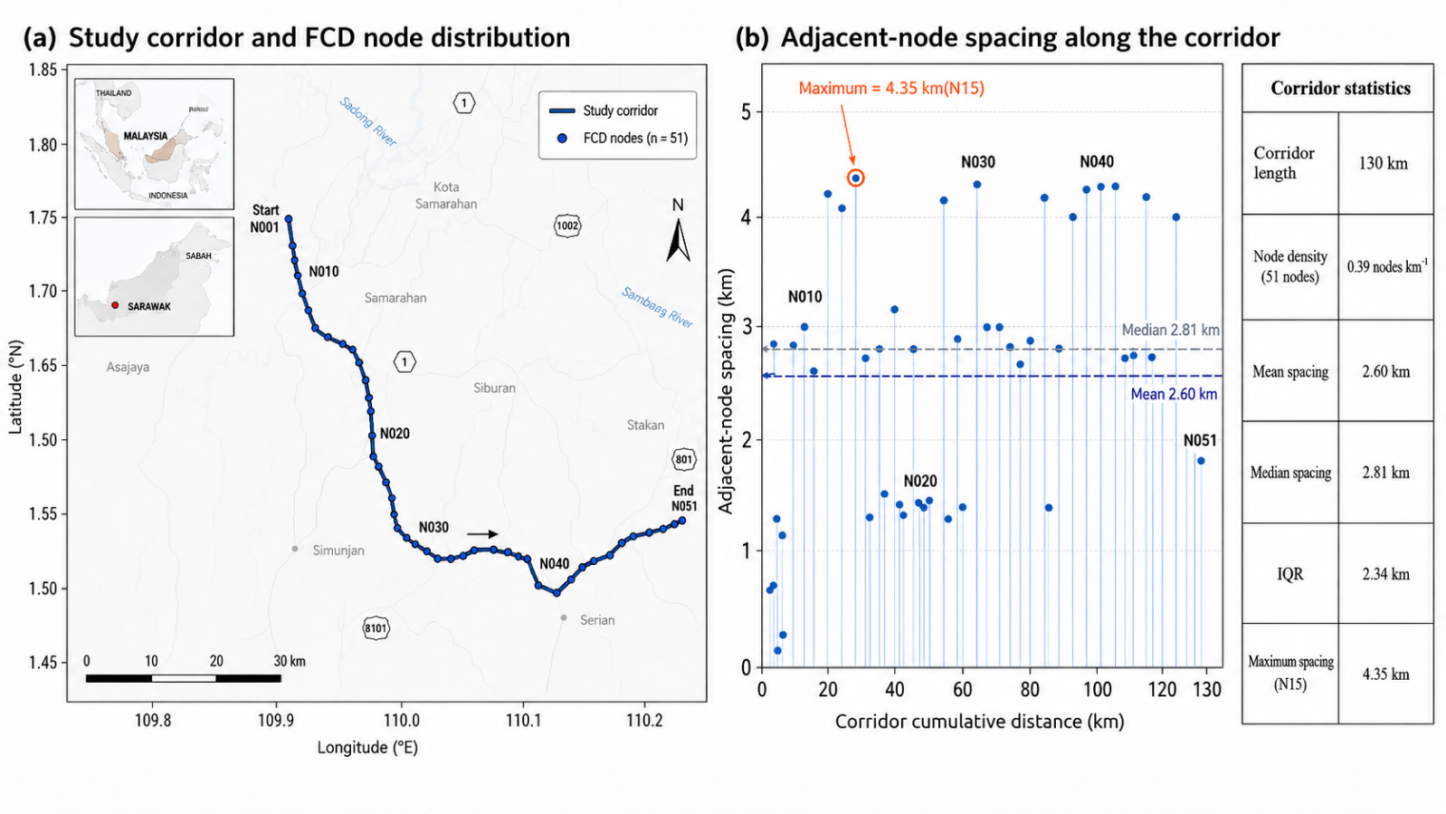
\includegraphics[width=0.92\textwidth]{Fig1.png}
    \caption{Study corridor and spatial configuration of the 51 FCD observation nodes. Panel (a) shows the approximately 130-km Pan Borneo Highway study corridor and the sequential distribution of nodes N01--N51. Panel (b) summarizes the spacing between adjacent nodes. The nodes represent discrete FCD observation locations rather than continuous sensing along the corridor}
    \label{fig:study_corridor}

    \figurenote{Nodes N01--N51 are fixed virtual FCD observation locations, and panel (b) reports the spacing of the 50 adjacent-node intervals. The map provides spatial context only; it does not imply continuous sensing between neighboring nodes.}
\end{figure}


Traffic observations were obtained from the TomTom Traffic API. The service provides provider-processed traffic information at predefined virtual locations rather than raw trajectories of individual vehicles. The available records include current speed, free-flow speed, current and free-flow travel time, confidence information, and road-closure status. The forecasting target is \emph{FCD-reported speed}, which represents the speed estimated by the commercial provider from its upstream data and processing pipeline. It should not be interpreted as an independently measured ground-truth speed from a fixed detector. This distinction is retained throughout the study because the forecasting experiment evaluates the temporal predictability of the provider-reported traffic state rather than the measurement accuracy of the FCD service itself.

The raw FCD records span from 8 December 2025 at 13:15 to 28 February 2026 at 23:45 in the Asia/Kuala\_Lumpur time zone (UTC+08:00), with a planned temporal resolution of 15~min. The first raw records occur within the incomplete 13:00--14:00 boundary hour on 8 December 2025. This partial starting hour is retained in the raw-data provenance but excluded from the formal complete-bin panel used for hourly forecasting. Accordingly, the complete analysis grid begins at 14:00 on 8 December 2025 and extends through the final complete hour beginning at 23:00 on 28 February 2026. The construction of this complete temporal grid, its theoretical denominator, and the eligibility rules applied before hourly aggregation are defined in Section~\ref{subsec:eligibility}.

\subsection{Complete-grid reconstruction and data eligibility}
\label{subsec:eligibility}

Commercial FCD APIs return observed records rather than an explicit row for every planned node--time combination. Returned rows alone cannot be used as the denominator for completeness. Raw timestamps were expressed in Asia/Kuala\_Lumpur time (UTC+08:00) and floored to 15-min intervals. The raw series starts at 13:15 on 8 December 2025, but the 13:00--14:00 boundary hour is incomplete. The formal complete grid starts at 14:00 on 8 December 2025 and ends at 23:45 on 28 February 2026.

The complete period contains 7,912 planned 15-min intervals and 1,978 complete hourly intervals per node. With 51 fixed nodes, the two theoretical denominators are

\begin{equation}
N_{15}=51\times7{,}912=403{,}512,
\qquad
N_{\mathrm{hour}}=51\times1{,}978=100{,}878.
\label{eq:grid_denominators}
\end{equation}

Every planned node--quarter-hour combination remains in the reconstructed grid even when no usable API record was returned. An unreturned observation is represented explicitly as missing rather than disappearing from the denominator.

Returned records were screened before aggregation. A record was retained only when the frozen timestamp, coordinate, speed, travel-time, confidence, and general-validity checks passed; road closure was false; current travel time was finite and positive; speed satisfied $0<v\leq130$~km~h$^{-1}$; and provider confidence satisfied $0.80\leq c\leq1.00$. The raw input contained 244,477 records. Of these, 1,170 failed the confidence threshold, while none failed the positive-speed rule or exceeded 130~km~h$^{-1}$. The complete frozen filter retained 243,307 records. No separate provider-status field was available, so the provider traffic-state category was retained as descriptive information rather than used as an additional filter.

After filtering, records with the same node and floored quarter-hour key were collapsed by arithmetic mean. This produced 241,601 deduplicated 15-min records. Duplicate observations occurred in 1,580 node--quarter-hour groups, corresponding to 1,706 excess rows removed by aggregation.

Hourly speeds were then constructed from the four planned quarter-hour positions within each hour. For node $i$ and hour $t$,

\begin{equation}
x_{i,t}=\frac{\sum_{q=1}^{4} I_{i,t,q}v_{i,t,q}}{m_{i,t}},
\qquad
m_{i,t}=\sum_{q=1}^{4}I_{i,t,q},
\qquad
x_{i,t}\ \text{is retained iff }m_{i,t}\geq2,
\label{eq:hourly_aggregation}
\end{equation}

where $v_{i,t,q}$ is the eligible quarter-hour speed and $I_{i,t,q}\in\{0,1\}$ indicates whether that position contains an eligible observation. Under the primary 2-of-4 rule, 83,439 of the 100,878 theoretical node--hour combinations are observed and 17,439 remain missing, giving 82.71\% hourly coverage. The 1-of-4, 3-of-4, and 4-of-4 rules are retained only for sensitivity analysis. Table~\ref{tab:data_eligibility_protocol} summarizes the frozen data contract.

\begin{table}[!htbp]
\centering
\caption{Dataset and eligibility protocol for construction of the hourly FCD panel.}
\label{tab:data_eligibility_protocol}
\footnotesize
\begin{tabularx}{\textwidth}{|>{\raggedright\arraybackslash}p{0.23\textwidth}|>{\raggedright\arraybackslash}p{0.30\textwidth}|>{\raggedright\arraybackslash}X|}
\hline
\textbf{Component} & \textbf{Frozen definition} & \textbf{Result / purpose} \\
\hline
Raw observation window & 8 Dec 2025 13:15 to 28 Feb 2026 23:45; UTC+08:00 & Preserves the collected-data provenance. \\
\hline
Formal analysis grid & 8 Dec 2025 14:00 to 28 Feb 2026 23:45; 51 nodes & Excludes the incomplete starting hour. \\
\hline
Planned grid & 7,912 quarter-hours and 1,978 complete hours per node & 403,512 node--quarter-hours and 100,878 node--hours. \\
\hline
Record eligibility & Valid time, coordinates, speed, travel time, confidence and flags; road closure false; positive finite travel time; $0<v\leq130$~km~h$^{-1}$; $0.80\leq c\leq1.00$ & 244,477 raw records reduced to 243,307 eligible records; 1,170 fail confidence. \\
\hline
Duplicate handling & Arithmetic mean within identical node--quarter-hour keys after filtering & 241,601 deduplicated 15-min records; 1,580 duplicate groups. \\
\hline
Primary hourly rule & Mean of eligible quarter-hour speeds when at least 2 of 4 positions are observed & 83,439 observed and 17,439 missing node--hours; 82.71\% coverage. \\
\hline
Sensitivity rules & 1-of-4, 3-of-4, and 4-of-4 & Used only to assess coverage sensitivity. \\
\hline
Target semantics & Provider-reported FCD speed; no independent detector ground truth & Forecasting evaluates temporal predictability of the commercial traffic-state product. \\
\hline
\end{tabularx}
\end{table}

\subsection{Dataset characteristics}
\label{subsec:dataset-characteristics}

The reconstructed dataset shows an important distinction between descriptive FCD return availability and the stricter hourly coverage used for formal forecasting. The original availability view in Figure~\ref{fig:fcd-availability} summarizes whether FCD were returned across the expected node--time structure before the final primary 2-of-4 hourly eligibility rule was imposed. In that descriptive view, daily availability was generally high, with a mean of 97.30\%, a minimum of 94.21\%, and a maximum of 99.03\%. Missing returns were not distributed uniformly across days. Some days contained only 1--3 missing node--hour records, whereas more affected days contained more than 40, with a maximum of approximately 44. For a complete 24-h day, the descriptive reference count is 1,224 node--hour combinations (51 nodes $\times$ 24 h), and the observed count was usually close to this value, although several days decreased to approximately 1,179--1,190 records.

\begin{figure}[!htbp]
    \centering
    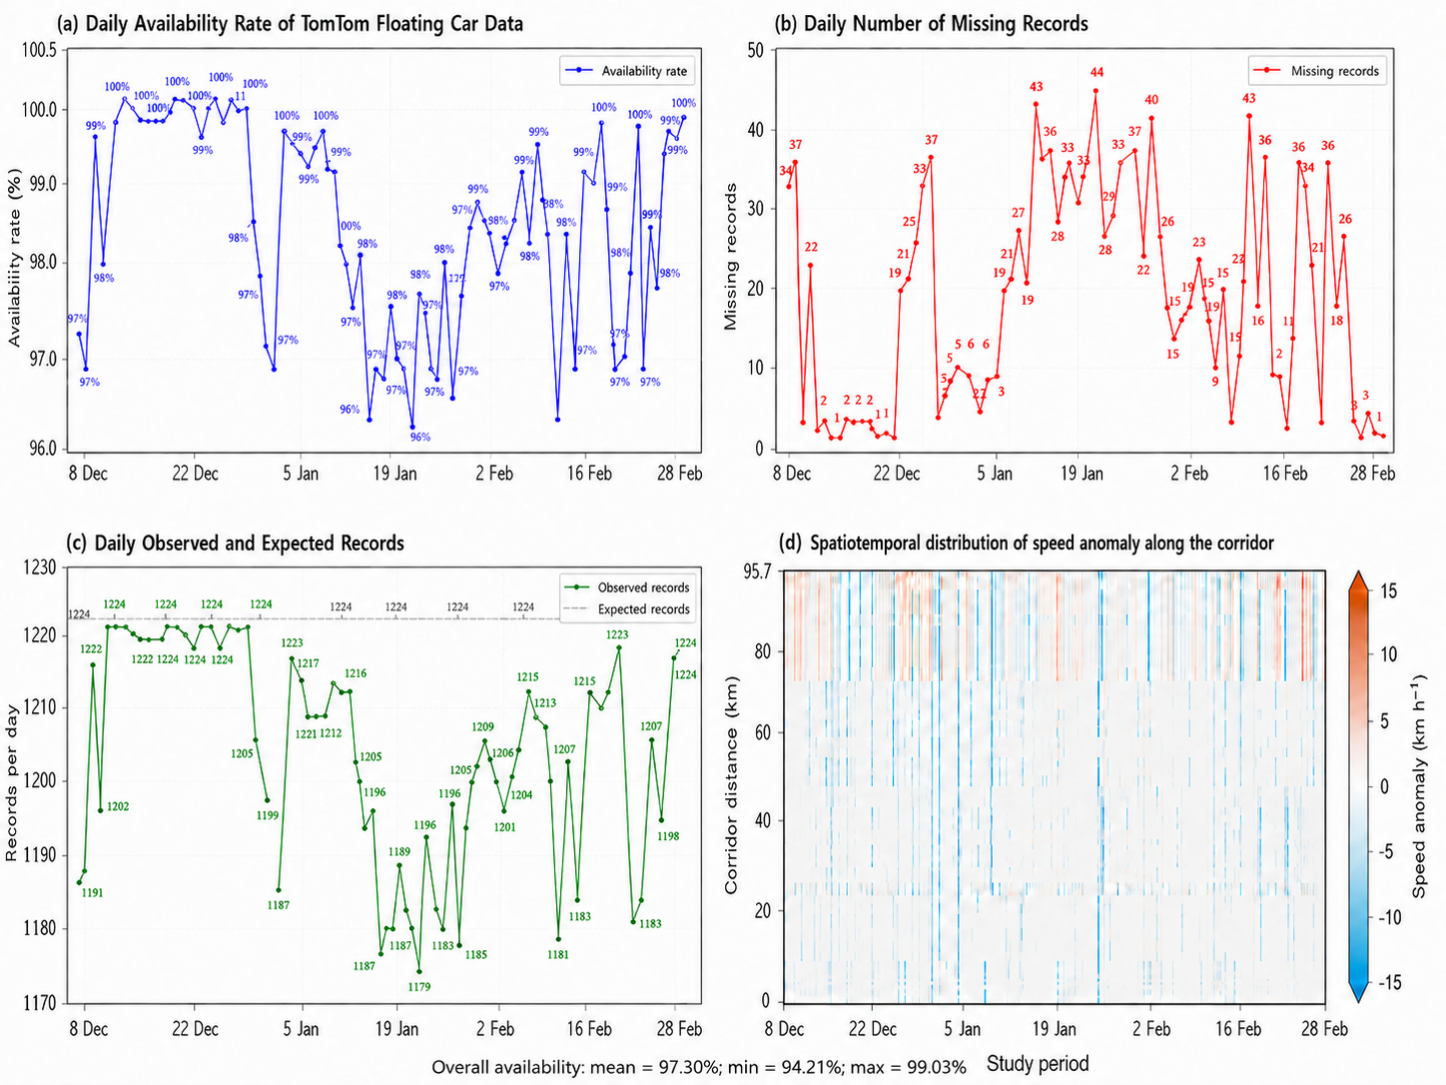
\includegraphics[width=0.92\textwidth]{Fig2.png}
    \caption{FCD availability, missingness, and speed variation during the study period. Panels (a)--(c) show descriptive return availability, missing returns, and observed versus expected daily records. Panel (d) shows corridor-wide signed speed deviations. This descriptive view is distinct from the primary 2-of-4 hourly eligibility used for forecasting}
    \label{fig:fcd-availability}

    \figurenote{Panels (a)--(c) describe raw return availability before the stricter 2-of-4 hourly eligibility rule is applied, whereas panel (d) shows signed corridor-wide speed deviations. The figure characterizes observation heterogeneity and traffic variation and is not used as evidence of forecasting accuracy.}
\end{figure}


The primary forecasting panel is more restrictive than the descriptive return-availability view because an hour is retained only when at least two quality-eligible 15-min observations are available. Under this 2-of-4 rule, 83,439 of the 100,878 theoretical node--hour combinations are observed, giving a formal hourly coverage of 82.71\%. The sensitivity thresholds show how strongly coverage depends on the required number of within-hour observations. A 1-of-4 rule retains 96,968 node--hour observations (96.12\%), whereas 3-of-4 and 4-of-4 retain 45,356 (44.96\%) and 15,838 (15.70\%), respectively. The main reduction in forecasting-eligible coverage therefore comes from the within-hour completeness requirement rather than from the complete disappearance of FCD returns.

Figure~\ref{fig:fcd-availability}(d) further indicates that speed variation is not spatially or temporally uniform along the corridor. The signed deviations shown in the original descriptive figure are approximately distributed between $-15$ and $+15$~km~h$^{-1}$ and occur at different dates and corridor positions. This panel is used only to characterize traffic heterogeneity; it is not used as a forecasting target, a model-selection criterion, or evidence of prediction performance. Despite the high basic return rate, the dataset remains spatially discrete, temporally incomplete, and heterogeneous. The next subsection therefore constructs causal histories while retaining descriptors of observation reliability.

\subsection{Causal preprocessing and feature construction}
\label{subsec:features}

The primary 2-of-4 panel contains explicit missing hourly speeds. Preprocessing is performed separately within each rolling-origin fold, with fallback values and scaling parameters estimated only from that fold's training interval. For node $i$ and forecast origin $t_0$, the input contains the origin hour and the preceding 23 h,

\begin{equation}
\mathcal{H}_{i,t_0}=\{t_0-23\mathrm{h},\ldots,t_0\},
\qquad |\mathcal{H}_{i,t_0}|=24.
\label{eq:history_window}
\end{equation}

All targets begin strictly after $t_0$. Historical state is not reset at train--validation--test boundaries because observations before an evaluation origin are legitimately available at that origin.

Missing input speeds were filled in two stages. A node-wise causal forward fill was applied first. If no earlier observed speed existed, the remaining leading missing value used a node median estimated from the fold-training interval; if that median was unavailable, the fold-training corridor median was used. Let $\tau_{i,t}$ be the latest earlier observed timestamp, $\eta_i^{(f)}$ the training-only node median, and $\eta_{\mathrm{corr}}^{(f)}$ the training-only corridor median. The model-ready speed is

\begin{equation}
\widetilde{x}_{i,t}^{(f)}=
\begin{cases}
x_{i,t}, & x_{i,t}\ \text{observed},\\
x_{i,\tau_{i,t}}, & \tau_{i,t}\ \text{exists},\\
\eta_i^{(f)}, & \tau_{i,t}\ \text{absent and }\eta_i^{(f)}\ \text{available},\\
\eta_{\mathrm{corr}}^{(f)}, & \text{otherwise}.
\end{cases}
\label{eq:causal_fill}
\end{equation}

No backward fill, centered rolling statistic, or future merge was used. The fallback medians and standardization parameters are fold-level quantities estimated once from the corresponding training interval; they are not re-estimated online at every timestamp.

Seven traffic-state and reliability descriptors were derived from the observed and filled hourly series. With $O_{i,t}$ denoting observed status, $M_{i,t}$ missing status, and $\mathcal{W}_{t}$ the trailing window of at most 24 hourly rows, the principal descriptors are

\begin{equation}
\begin{aligned}
O_{i,t}&=\mathbb{I}(x_{i,t}\ \text{observed}),\qquad M_{i,t}=1-O_{i,t},\\
\mathcal{W}_{t}&=\{\max(t_{\min},t-23\mathrm{h}),\ldots,t\},\qquad n_t=|\mathcal{W}_t|,\\
\mathrm{coverage}_{i,t}^{24}&=\frac{1}{n_t}\sum_{s\in\mathcal{W}_t}O_{i,s},\qquad
\mathrm{imputation}_{i,t}^{24}=1-\mathrm{coverage}_{i,t}^{24},\\
\overline{\widetilde{x}}_{i,t}^{(f)}&=\frac{1}{n_t}\sum_{s\in\mathcal{W}_t}\widetilde{x}_{i,s}^{(f)},\\
\mathrm{volatility}_{i,t}^{24,(f)}&=
\begin{cases}
\sqrt{\frac{1}{n_t}\sum_{s\in\mathcal{W}_t}\left(\widetilde{x}_{i,s}^{(f)}-\overline{\widetilde{x}}_{i,t}^{(f)}\right)^2}, & n_t\ge2,\\
0, & n_t=1.
\end{cases}
\end{aligned}
\label{eq:reliability_descriptors}
\end{equation}

The remaining reliability descriptors are the current-hour missing/imputation indicator, the elapsed hours since the most recent observation (capped at 168 h), and the longest missing run in the trailing 24-h window. Calendar information is represented by sine and cosine encodings of hour of day and day of week plus a weekend indicator. The rolling volatility in Eq.~\eqref{eq:reliability_descriptors} is the population standard deviation of the causally filled speed (\texttt{ddof=0}), not a mean absolute change. Table~\ref{tab:feature_set} lists the frozen 13-feature sequence.

\begin{table}[!htbp]
\centering
\caption{Frozen 13-feature sequence for each hourly history row.}
\label{tab:feature_set}
\footnotesize
\begin{tabularx}{\textwidth}{|>{\centering\arraybackslash}p{0.05\textwidth}|>{\raggedright\arraybackslash}p{0.32\textwidth}|>{\raggedright\arraybackslash}X|}
\hline
\textbf{No.} & \textbf{Feature} & \textbf{Definition} \\
\hline
1 & \texttt{input\_speed\_filled} & Observed hourly speed after causal forward fill and training-only fallback. \\
\hline
2 & \texttt{hourly\_missing\_mask} & 1 when the primary hourly speed is missing; 0 otherwise. \\
\hline
3 & \texttt{imputed\_flag} & 1 when the model input speed is filled; numerically identical to the missing mask in the frozen pipeline. \\
\hline
4 & \texttt{hours\_since\_last\_observation} & Elapsed hourly grid steps since the most recent observation; 0 when observed and capped at 168 h. \\
\hline
5 & \texttt{history\_coverage\_ratio} & Observed fraction in the trailing window of at most 24 h. \\
\hline
6 & \texttt{history\_imputation\_ratio} & One minus the history-coverage ratio. \\
\hline
7 & \texttt{max\_gap\_24h} & Longest consecutive missing run within the trailing window. \\
\hline
8 & \texttt{volatility\_24h} & Population SD of the filled speed within the trailing window. \\
\hline
9 & \texttt{hour\_sin} & Sine encoding of hour of day. \\
\hline
10 & \texttt{hour\_cos} & Cosine encoding of hour of day. \\
\hline
11 & \texttt{dow\_sin} & Sine encoding of day of week. \\
\hline
12 & \texttt{dow\_cos} & Cosine encoding of day of week. \\
\hline
13 & \texttt{weekend\_flag} & 1 for Saturday or Sunday; 0 otherwise. \\
\hline
\end{tabularx}
\end{table}

All 13 sequence features were standardized separately within each fold using the fold-training mean and population standard deviation. For feature $c$,

\begin{equation}
z_{c,i,t}^{(f)}=\frac{u_{c,i,t}^{(f)}-\mu_c^{(f)}}{s_c^{(f)}},
\label{eq:feature_standardization}
\end{equation}

where a fitted zero standard deviation is replaced by 1. Validation and test rows use the frozen training parameters and do not contribute to fitting. The sequential representation is $24\times13$. For tabular models, the standardized sequence is flattened to 312 values and concatenated with node order, latitude, and longitude, yielding a 315-dimensional vector. Sequence and tabular inputs are generated from the same forecast origins and frozen sample identifiers.

% ======================================================================
% 4 FORECASTING MODELS
% ======================================================================

\section{Forecasting models}
\label{sec:models}

Figure~\ref{fig:gate-fcd-framework} summarizes the GATE-FCD workflow from complete-grid reconstruction to common-sample evaluation and audit. This section defines the three forecasting tasks and the six frozen models; Section~\ref{sec:evaluation} describes the rolling-origin evaluation and statistical analysis.

\begin{figure}[!htbp]
    \centering
    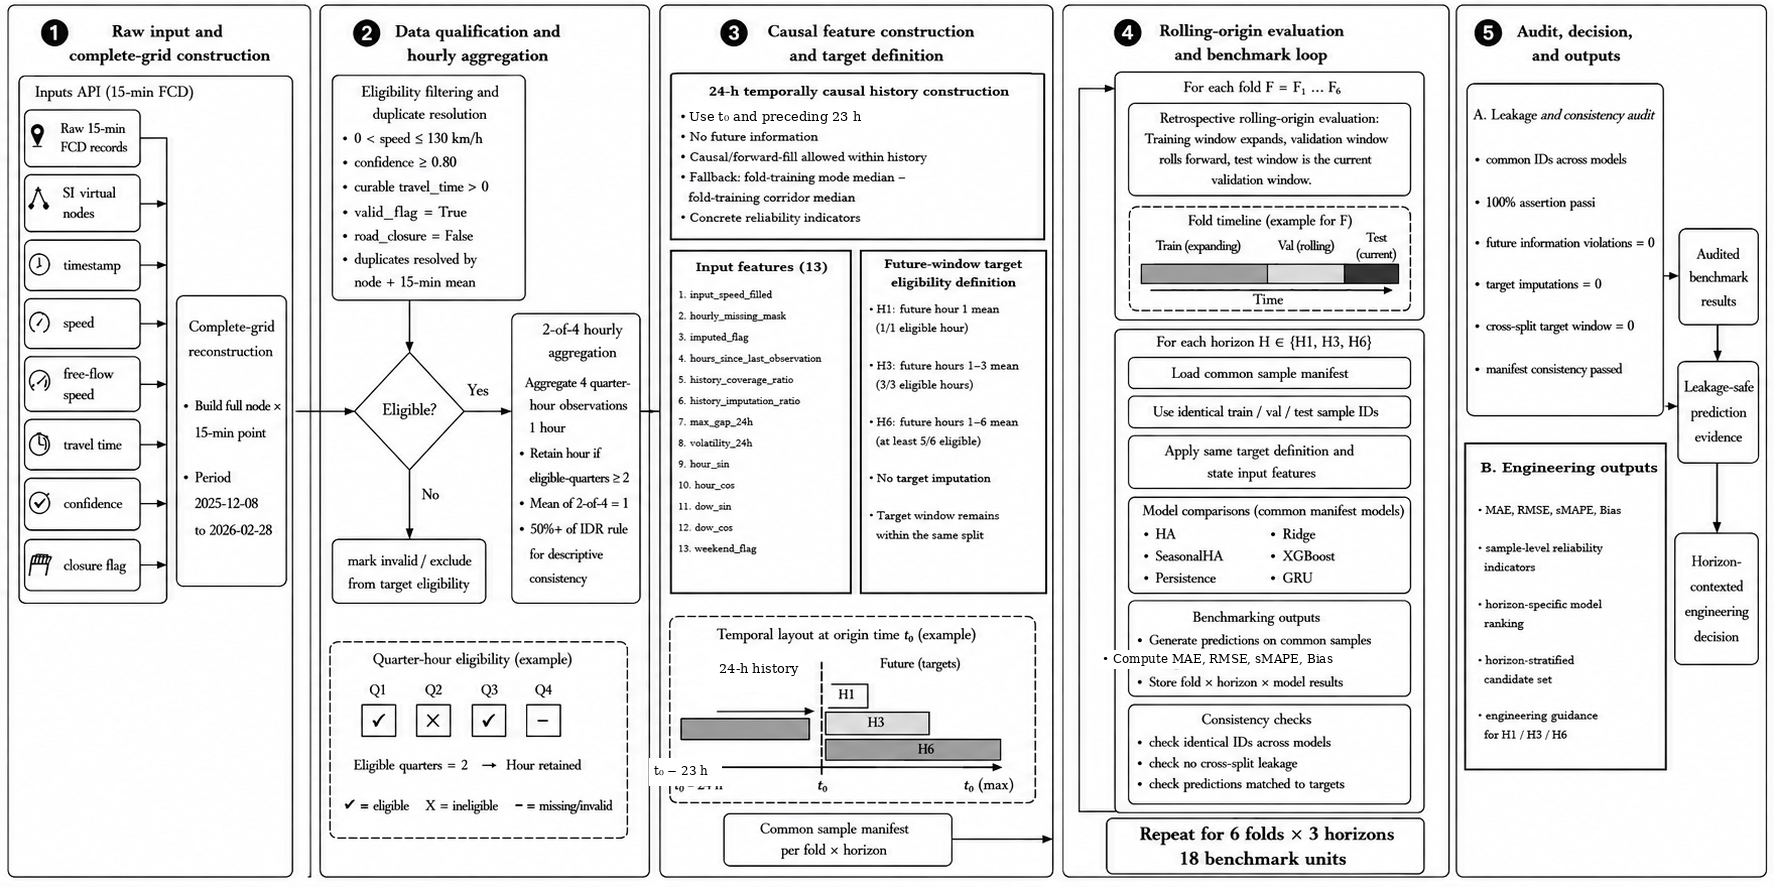
\includegraphics[width=0.97\textwidth]{Fig3.png}
    \caption{GATE-FCD multi-horizon forecasting framework. The workflow links complete-grid reconstruction and hourly eligibility, causal feature construction and future-window targets, six-fold rolling-origin model comparison on common samples, and final audit and interpretation}
    \label{fig:gate-fcd-framework}

    \figurenote{Arrows denote the ordered evidence-construction workflow from reconstructed observations to audited forecasts, not causal relationships among traffic variables. All six candidate models enter only after eligibility, temporal-causality, and common-manifest constraints have been fixed.}
\end{figure}

\subsection{Multi-horizon forecasting tasks}
\label{subsec:tasks}

For node $i$ and forecast origin $t_0$, the 24-h input history ends at $t_0$ and every target hour occurs after the origin. Three horizons are evaluated, $H\in\{1,3,6\}$~h, and each is defined as a future-window mean rather than a point forecast exactly at $t_0+H$. Multi-horizon traffic forecasting is commonly formulated with horizon-specific prediction targets and evaluation tasks \cite{Hadry2025TrafficForecasting,Zeb2024FeatureProjection}. Following this principle, the present study defines a study-specific future-window mean target with an explicit completeness gate. Let $\mathcal{F}_{i,t_0}^{(H)}$ be the planned future window and $\mathcal{O}_{i,t_0}^{(H)}$ its observed subset:

\begin{equation}
\begin{aligned}
\mathcal{F}_{i,t_0}^{(H)}&=\{t_0+1\mathrm{h},\ldots,t_0+H\mathrm{h}\},\\
\mathcal{O}_{i,t_0}^{(H)}&=\{s\in\mathcal{F}_{i,t_0}^{(H)}:x_{i,s}\ \text{observed}\},\\
q_H&=\begin{cases}1,&H=1,\\3,&H=3,\\5,&H=6,\end{cases}
\qquad |\mathcal{O}_{i,t_0}^{(H)}|\ge q_H,\\
y_{i,t_0}^{(H)}&=\frac{1}{|\mathcal{O}_{i,t_0}^{(H)}|}
\sum_{s\in\mathcal{O}_{i,t_0}^{(H)}}x_{i,s}.
\end{aligned}
\label{eq:target_contract}
\end{equation}

Thus, H1 requires 1/1 observed future hour, H3 requires 3/3, and the primary H6 task requires at least 5/6. Target values are never imputed. The complete target window must remain inside the same train, validation, or test split as its forecast origin; boundary-crossing origins are excluded. A stricter H6 6-of-6 rule is retained only as sensitivity analysis. Table~\ref{tab:target_definitions} summarizes the three target contracts.

\begin{table}[!htbp]
\centering
\caption{Primary future-window mean-speed target definitions.}
\label{tab:target_definitions}
\small
\begin{tabularx}{\textwidth}{|>{\centering\arraybackslash}p{0.07\textwidth}|>{\raggedright\arraybackslash}p{0.18\textwidth}|>{\raggedright\arraybackslash}p{0.17\textwidth}|>{\raggedright\arraybackslash}X|>{\centering\arraybackslash}p{0.13\textwidth}|}
\hline
\textbf{Task} & \textbf{Future window} & \textbf{Observed-hour rule} & \textbf{Target} & \textbf{Equation} \\
\hline
H1 & $t_0+1$~h & 1 of 1 & Speed in the next observed hour. & Eq.~\eqref{eq:target_contract} \\
\hline
H3 & $t_0+1$ to $t_0+3$~h & 3 of 3 & Mean of all three future hourly speeds. & Eq.~\eqref{eq:target_contract} \\
\hline
H6 & $t_0+1$ to $t_0+6$~h & At least 5 of 6 & Mean of the 5 or 6 observed future hourly speeds; no target imputation. & Eq.~\eqref{eq:target_contract} \\
\hline
\end{tabularx}
\end{table}

Because the targets average windows of different lengths, raw error magnitudes are interpreted primarily within each horizon. A lower H6 MAE than H1 MAE does not imply that six-hour forecasting is intrinsically easier; the longer window can smooth short-term variation.

\subsection{Naive and statistical baselines}
\label{subsec:baselines}

HA, SeasonalHA, Persistence, and Ridge provide deterministic references with increasing flexibility. Historical-average, seasonal-average, and persistence predictors are standard reference baselines in time-series forecast evaluation and are also used in traffic-forecasting comparisons \cite{Hewamalage2023ForecastEvaluation,Hadry2025TrafficForecasting}. For fold $f$ and horizon $H$, let $\mathcal{T}_{f,H}$ denote the eligible training cases and $\mathcal{S}_{f,H}(t_0)$ the frozen seasonal subset matched to the target time. Under the common-manifest design, the three nonparametric baselines are

\begin{equation}
\begin{aligned}
\widehat{y}_{f,H}^{\mathrm{HA}}&=\frac{1}{|\mathcal{T}_{f,H}|}\sum_{j\in\mathcal{T}_{f,H}}y_j^{(H)},\\
\widehat{y}_{i,t_0}^{\mathrm{SeasonalHA},(f,H)}&=\frac{1}{|\mathcal{S}_{f,H}(t_0)|}\sum_{j\in\mathcal{S}_{f,H}(t_0)}y_j^{(H)},\\
\widehat{y}_{i,t_0}^{\mathrm{Persistence},(H)}&=\widetilde{x}_{i,t_0}^{(f)}.
\end{aligned}
\label{eq:baseline_models}
\end{equation}

HA represents the overall target level, SeasonalHA recurring calendar structure, and Persistence current-state continuity. For a fixed node and origin, Persistence produces the same numerical forecast at H1, H3, and H6; only the target window changes.

Ridge is the learned linear benchmark. Ridge regression augments least-squares estimation with an $L_2$ penalty to stabilize coefficient estimation when predictors are correlated \cite{HoerlKennard1970Ridge}. With $\mathbf{z}_{j}^{(f)}\in\mathbb{R}^{315}$ denoting the tabular input, the fold--horizon model is fitted by

\begin{equation}
(\widehat{\beta}_{0}^{(f,H)},\widehat{\boldsymbol{\beta}}^{(f,H)})
=\arg\min_{\beta_0,\boldsymbol{\beta}}
\left[\sum_{j\in\mathcal{T}_{f,H}}
\left(y_j^{(H)}-\beta_0-\mathbf{z}_{j}^{(f)\top}\boldsymbol{\beta}\right)^2
+\alpha\|\boldsymbol{\beta}\|_2^2\right],
\qquad \alpha=1.0.
\label{eq:ridge}
\end{equation}

The intercept is not penalized. Ridge tests whether the common traffic-state, reliability, calendar, and node features provide useful approximately linear predictive information.

\subsection{Machine-learning and deep-learning models}
\label{subsec:ml-dl}

XGBoost and GRU represent nonlinear tabular learning and recurrent sequence learning. Both use the same frozen cases and targets as the baselines. XGBoost is based on additive gradient-boosted regression trees, in which the final prediction is the sum of the outputs from the fitted trees \cite{ChenGuestrin2016XGBoost}. For the 315-dimensional input used here, the prediction is written as

\begin{equation}
\widehat{y}_{j}^{\mathrm{XGB}}=\sum_{b=1}^{500}f_b(\mathbf{z}_j).
\label{eq:xgboost_prediction}
\end{equation}

The frozen configuration uses maximum depth 8, learning rate 0.05, row subsampling 0.8, column subsampling 0.8, the \texttt{reg:squarederror} objective, \texttt{tree\_method=hist}, and 10 central processing unit (CPU) jobs. No model-specific feature selection is applied after the common input representation is frozen.

GRU receives the standardized $24\times13$ sequence. The recurrent state follows the gated recurrent unit architecture introduced for sequence modeling by Cho et al. \cite{Cho2014GRU}; the present implementation uses the final hidden state for scalar speed prediction. Its input, recurrent update, and output are

\begin{equation}
\begin{aligned}
\mathbf{X}_{j}&=[\mathbf{x}_{j,1},\ldots,\mathbf{x}_{j,24}]^{\top}\in\mathbb{R}^{24\times13},\\
\mathbf{h}_{j,\tau}&=\operatorname{GRU}_{\theta}(\mathbf{x}_{j,\tau},\mathbf{h}_{j,\tau-1}),\qquad \tau=1,\ldots,24,\\
\widehat{y}_{j}^{\mathrm{GRU}}&=\mathbf{w}_{o}^{\top}\mathbf{h}_{j,24}+b_o.
\end{aligned}
\label{eq:gru_model}
\end{equation}

The frozen GRU has one recurrent layer, hidden size 64, and dropout 0.0. Training uses batch size 256, learning rate $10^{-3}$, weight decay $10^{-4}$, gradient clipping at norm 1.0, and at most 30 epochs. Early stopping monitors validation mean absolute error (MAE) with patience 5 and \texttt{minimum\_delta=0.0}; the checkpoint with the lowest validation MAE is retained.

XGBoost and GRU are repeated with seeds 42, 2026, and 3407. Prediction averaging across repeated learners is a standard ensemble strategy and has been used to improve stability in traffic forecasting \cite{Cini2024DeepEnsemble}. Here, the three seed-level predictions are averaged at the sample level before metric calculation:

\begin{equation}
\overline{\widehat{y}}_{j}^{(M,f,H)}=\frac{1}{3}\sum_{s\in\{42,2026,3407\}}\widehat{y}_{j,s}^{(M,f,H)},
\qquad
e_j^{(M,f,H)}=\overline{\widehat{y}}_{j}^{(M,f,H)}-y_j^{(H)},
\label{eq:seed_ensemble}
\end{equation}

for $M\in\{\mathrm{XGBoost},\mathrm{GRU}\}$. Seed-specific predictions are retained for the stability analysis. Table~\ref{tab:model_protocol} summarizes the frozen model configurations and their experimental roles.

\begin{table}[!htbp]
\centering
\caption{Frozen forecasting models and experimental roles.}
\label{tab:model_protocol}
\footnotesize
\begin{tabularx}{\textwidth}{|>{\raggedright\arraybackslash}p{0.11\textwidth}|>{\raggedright\arraybackslash}p{0.17\textwidth}|>{\raggedright\arraybackslash}p{0.29\textwidth}|>{\raggedright\arraybackslash}X|>{\centering\arraybackslash}p{0.15\textwidth}|}
\hline
\textbf{Model} & \textbf{Primary input} & \textbf{Frozen rule / setting} & \textbf{Role} & \textbf{Equation(s)} \\
\hline
HA & Fold--horizon training targets & Arithmetic mean; deterministic & Overall mean reference. & Eq.~\eqref{eq:baseline_models} \\
\hline
SeasonalHA & Seasonally matched training targets & Mean of the frozen seasonal reference set; deterministic & Calendar-pattern reference. & Eq.~\eqref{eq:baseline_models} \\
\hline
Persistence & Filled speed at $t_0$ & No fitted parameters & Current-state reference. & Eq.~\eqref{eq:baseline_models} \\
\hline
Ridge & 315-dimensional vector & L2 regression; $\alpha=1.0$ & Learned linear benchmark. & Eq.~\eqref{eq:ridge} \\
\hline
XGBoost & 315-dimensional vector & 500 trees; depth 8; learning rate 0.05; subsample 0.8; column subsample 0.8; three seeds & Nonlinear tabular benchmark. & Eqs.~\eqref{eq:xgboost_prediction}, \eqref{eq:seed_ensemble} \\
\hline
GRU & $24\times13$ sequence & One layer; hidden 64; batch 256; learning rate $10^{-3}$; weight decay $10^{-4}$; max 30 epochs; patience 5; three seeds & Recurrent benchmark. & Eqs.~\eqref{eq:gru_model}, \eqref{eq:seed_ensemble} \\
\hline
\end{tabularx}
\end{table}

% ======================================================================
% 5 EVALUATION
% ======================================================================

\section{Evaluation}
\label{sec:evaluation}

\subsection{Experimental setup}
\label{subsec:setup}

The formal experiment uses six retrospective rolling-origin folds and the three forecasting horizons H1, H3, and H6 defined in Section~\ref{subsec:tasks}. The evaluation is explicitly retrospective rather than an independent blind test. The fold schedule preserves chronological train--validation--test ordering, but the terminal evaluation period had been exposed during earlier model-development work. Consequently, the present results are interpreted as repeated out-of-time evidence under a frozen protocol, and no independent blind-test claim is made. This distinction is retained throughout the paper even though the formal configuration prohibited result-driven model changes and future-information use during the frozen rerun.

Table~\ref{tab:rolling_folds} gives the exact temporal boundaries. All intervals are expressed in local time (Asia/Kuala\_Lumpur, UTC+08:00) and use half-open notation $[\mathrm{start},\mathrm{end})$. The training interval expands by one week from Fold~1 to Fold~6, while validation and test windows advance chronologically. The formal fold schedule starts on 9 December 2025 at 00:00. Earlier complete-grid hours remain part of the reconstructed data provenance but are not assigned as formal forecast origins in this fold schedule.

\begin{table}[!htbp]
\centering
\caption{Frozen retrospective rolling-origin fold schedule. Interval end times are exclusive.}
\label{tab:rolling_folds}
\footnotesize
\begin{tabularx}{\textwidth}{|>{\centering\arraybackslash}p{0.07\textwidth}|>{\raggedright\arraybackslash}p{0.29\textwidth}|>{\raggedright\arraybackslash}p{0.27\textwidth}|>{\raggedright\arraybackslash}X|}
\hline
\textbf{Fold} &
\textbf{Training interval} &
\textbf{Validation interval} &
\textbf{Test interval} \\
\hline
1 & 9 Dec 2025 00:00--12 Jan 2026 00:00 & 12 Jan 2026 00:00--19 Jan 2026 00:00 & 19 Jan 2026 00:00--26 Jan 2026 00:00 \\ 
\hline
2 & 9 Dec 2025 00:00--19 Jan 2026 00:00 & 19 Jan 2026 00:00--26 Jan 2026 00:00 & 26 Jan 2026 00:00--2 Feb 2026 00:00 \\ 
\hline
3 & 9 Dec 2025 00:00--26 Jan 2026 00:00 & 26 Jan 2026 00:00--2 Feb 2026 00:00 & 2 Feb 2026 00:00--9 Feb 2026 00:00 \\ 
\hline
4 & 9 Dec 2025 00:00--2 Feb 2026 00:00 & 2 Feb 2026 00:00--9 Feb 2026 00:00 & 9 Feb 2026 00:00--16 Feb 2026 00:00 \\ 
\hline
5 & 9 Dec 2025 00:00--9 Feb 2026 00:00 & 9 Feb 2026 00:00--16 Feb 2026 00:00 & 16 Feb 2026 00:00--23 Feb 2026 00:00 \\ 
\hline
6 & 9 Dec 2025 00:00--16 Feb 2026 00:00 & 16 Feb 2026 00:00--23 Feb 2026 00:00 & 23 Feb 2026 00:00--1 Mar 2026 00:00 \\
\hline
\multicolumn{4}{|p{0.965\textwidth}|}{\textit{Equation reference:} the future target must remain wholly inside the assigned split under Eq.~\eqref{eq:target_contract}; all intervals use the half-open convention $[\mathrm{start},\mathrm{end})$.} \\
\hline
\end{tabularx}
\end{table}


Each fold is crossed with three horizons, producing $6\times3=18$ fold--horizon benchmark units. Before model comparison, one common sample manifest is frozen for every unit. Each manifest fixes the eligible sample identifiers, node, forecast origin, split membership, and target definition used by all six models. The manifest registry stores an independent SHA-256 hash for each fold--horizon unit. The complete formal campaign contains 180 model runs: 72 deterministic runs from HA, SeasonalHA, Persistence, and Ridge, and 108 stochastic runs from XGBoost and GRU across three seeds. All 180 formal runs completed successfully, no run failed, and 180 prediction files were registered.

The formal campaign was executed on a 64-bit Windows local workstation using CPython~3.10. The recorded deep-learning environment used CUDA-enabled PyTorch on an NVIDIA RTX A3000 Laptop graphics processing unit (GPU). The analysis stack included NumPy, pandas, PyArrow, scikit-learn, XGBoost, PyTorch, and SciPy. The archived environment documentation preserves the principal software stack but not a complete final microversion and CUDA-version snapshot. Unverified package versions are not inferred in this paper. Reproducibility is instead anchored to the frozen configuration, Git revision, sample-manifest hashes, prediction-file hashes, and public audit materials.

\subsection{Rolling-origin evaluation and common-sample benchmarking}
\label{subsec:rolling}

Common manifests hold sample composition fixed while model behavior is compared. For each fold $f$ and horizon $H$, eligibility is resolved before any model is compared. A forecast case enters the manifest only when its 24-h input sequence can be constructed under the frozen preprocessing rules, its target satisfies the H1/H3/H6 observation requirement, and the full target window remains inside the assigned split. The resulting manifest stores a unique sample identifier together with node, forecast origin, split, target, and lineage fields. The same manifest is then used by HA, SeasonalHA, Persistence, Ridge, XGBoost, and GRU.

Across all 18 fold--horizon manifests, the registry contains 1,053,618 sample records: 873,874 training records, 87,597 validation records, and 92,147 test records. The six test windows contain 38,201 H1 cases, 24,805 H3 cases, and 29,141 H6 cases. These counts describe experimental scale rather than independent statistical replication because the expanding training windows overlap in time and observations within the same test period are temporally and spatially dependent.

The frozen sample audit checks sample alignment and temporal causality. All 20 full-sample assertions passed across the manifest registry. The checks confirm unique sample identifiers, 24-row histories, strictly increasing history timestamps, histories at or before the forecast origin, targets strictly after the origin, targets fully inside the assigned split, no target imputation, no history--target overlap, node consistency, target recomputation from source row identifiers, H1/H3/H6 coverage rules, training-only scalers and fallback medians, no backward fill, no centered rolling statistic, no future merge, and use of a common manifest by all models. Future-information violations, target-recomputation mismatches, and cross-split target-window violations were all zero. Table~\ref{tab:audit_scale} summarizes the experimental scale and audit outcomes; the full assertion list is provided in Appendix~\ref{app:audit}.

\begin{table}[!htbp]
\centering
\caption{Formal experimental scale and sample-audit summary.}
\label{tab:audit_scale}
\small
\begin{tabularx}{\textwidth}{|>{\raggedright\arraybackslash}p{0.42\textwidth}|>{\raggedright\arraybackslash}X|}
\hline
\textbf{Audit or scale item} & \textbf{Formal result} \\
\hline
Common fold--horizon manifests & 18; target eligibility follows Eq.~\eqref{eq:target_contract} \\ 
\hline
Formal model runs & 180/180 completed; 0 failed; stochastic predictions are aggregated by Eq.~\eqref{eq:seed_ensemble} \\ 
\hline
Total manifest records & 1,053,618 \\ 
\hline
Training / validation / test records & 873,874 / 87,597 / 92,147 \\ 
\hline
Test records by horizon & H1: 38,201; H3: 24,805; H6: 29,141 \\ 
\hline
Full-sample leakage and consistency assertions & 20/20 PASS \\ 
\hline
Future-information violations & 0 \\ 
\hline
Target-recomputation mismatches & 0 \\ 
\hline
Cross-split target-window violations & 0; split containment is part of Eq.~\eqref{eq:target_contract} \\ 
\hline
Primary inferential unit & Rolling-origin fold ($n=6$); paired effect defined by Eq.~\eqref{eq:paired_delta} \\ 
\hline
Evidence level & Retrospective rolling-origin; independent blind-test claim not made \\
\hline
\end{tabularx}
\end{table}


\subsection{Evaluation metrics and statistical analysis}
\label{subsec:metrics}

Mean absolute error (MAE) is the primary metric because it remains directly interpretable in km~h$^{-1}$. Root mean squared error (RMSE), symmetric mean absolute percentage error (sMAPE), and signed Bias are secondary checks. These error measures are standard in forecast evaluation and have been used in multi-horizon traffic-forecasting comparisons \cite{Hewamalage2023ForecastEvaluation,Hadry2025TrafficForecasting}. For a common test set of size $n$, with target $y_j$, prediction $\widehat{y}_j$, and error $e_j=\widehat{y}_j-y_j$,

\begin{equation}
\begin{aligned}
\mathrm{MAE}&=\frac{1}{n}\sum_{j=1}^{n}|e_j|,\qquad
\mathrm{RMSE}=\sqrt{\frac{1}{n}\sum_{j=1}^{n}e_j^2},\\
\mathrm{sMAPE}&=\frac{100}{n}\sum_{j=1}^{n}\frac{2|y_j-\widehat{y}_j|}{|y_j|+|\widehat{y}_j|+\varepsilon},\qquad
\mathrm{Bias}=\frac{1}{n}\sum_{j=1}^{n}(\widehat{y}_j-y_j),
\end{aligned}
\label{eq:evaluation_metrics}
\end{equation}

where $\varepsilon>0$ is the fixed numerical constant that prevents a zero sMAPE denominator. For XGBoost and GRU, these metrics use the three-seed sample-level average in Eq.~\eqref{eq:seed_ensemble}; seed-specific results are analyzed separately.

The six rolling-origin folds are the primary paired inferential units; node--time rows within a test period are not treated as independent replications. Dependence-aware forecast comparison should use paired evaluation units rather than treating correlated forecast errors as independent replications \cite{Hewamalage2023ForecastEvaluation}. For models $A$ and $B$, the study-specific paired fold-level effect is defined as

\begin{equation}
\Delta_{A,B}^{(f,H)}=\mathrm{MAE}_{A,f,H}-\mathrm{MAE}_{B,f,H},
\label{eq:paired_delta}
\end{equation}

so negative values favor model $A$. Five comparisons were prespecified within each horizon: XGBoost--GRU, XGBoost--Ridge, XGBoost--SeasonalHA, Persistence--HA, and GRU--Ridge. For each comparison, the frozen pipeline applies a two-sided Wilcoxon signed-rank test to the six paired fold-level MAE differences and uses 10,000 paired-bootstrap resamples to form an unadjusted 95\% confidence interval. The five p-values are then adjusted separately within each horizon using the Holm procedure \cite{GarciaPerez2023MultipleTesting}, yielding 15 prespecified comparisons in total. With only six paired folds per horizon, non-significance is interpreted as insufficient evidence of a stable difference rather than proof of equivalence.

A supplementary dependence-aware analysis uses 10,000 day$\times$spatial-block bootstrap replicates. Forty-one test days are crossed with five spatial blocks, producing 205 day--block clusters. Because this estimator changes the weighting and dependence structure relative to the fold-macro analysis, it is treated as supplementary uncertainty evidence rather than a second winner-selection procedure \cite{Hewamalage2023ForecastEvaluation}.

\subsection{Multi-horizon forecasting results}
\label{subsec:overall-results}

Table~\ref{tab:main_mae} and Figure~\ref{fig:performance_stability}(a--b) report the primary descriptive results. XGBoost had the lowest six-fold mean MAE at all three horizons: $0.949\pm0.258$, $0.829\pm0.168$, and $0.752\pm0.142$~km~h$^{-1}$ for H1, H3, and H6, respectively. SeasonalHA was close at $0.961\pm0.115$, $0.853\pm0.105$, and $0.774\pm0.102$~km~h$^{-1}$. The XGBoost--SeasonalHA gaps were $-0.0117$, $-0.0235$, and $-0.0222$~km~h$^{-1}$, or approximately 1.2\%, 2.8\%, and 2.9\% of the SeasonalHA MAE. This mean ranking is descriptive; its stability is assessed from the fold-level and uncertainty analyses below.

Persistence changed most strongly with horizon. Its H1 mean MAE was $0.950\pm0.155$~km~h$^{-1}$, essentially the same as XGBoost and slightly below SeasonalHA, but the value rose to $1.170\pm0.136$ at H3 and $1.470\pm0.182$~km~h$^{-1}$ at H6. Carrying the latest model-ready speed forward is thus a useful H1 reference but loses competitiveness as the target window lengthens. GRU recorded $1.151$, $1.043$, and $0.958$~km~h$^{-1}$ and Ridge $1.225$, $1.131$, and $1.086$~km~h$^{-1}$ at H1/H3/H6; neither entered the leading descriptive tier. HA had the highest or near-highest errors at all three horizons.

\begin{table}[!htbp]
\centering
\caption{Fold-macro MAE of the six forecasting models. Values are mean $\pm$ sample standard deviation across six retrospective rolling-origin folds, in km~h$^{-1}$.}
\label{tab:main_mae}
\small
\begin{tabular}{|l|c|c|c|}
\hline
\textbf{Model} & \textbf{H1} & \textbf{H3} & \textbf{H6} \\
\hline
\multicolumn{4}{|l|}{\textit{Metric definition:} MAE is defined in Eq.~\eqref{eq:evaluation_metrics}.} \\
\hline
XGBoost     & $0.949\pm0.258$ & $0.829\pm0.168$ & $0.752\pm0.142$ \\ 
\hline
SeasonalHA  & $0.961\pm0.115$ & $0.853\pm0.105$ & $0.774\pm0.102$ \\ 
\hline
Persistence & $0.950\pm0.155$ & $1.170\pm0.136$ & $1.470\pm0.182$ \\ 
\hline
GRU         & $1.151\pm0.230$ & $1.043\pm0.195$ & $0.958\pm0.199$ \\ 
\hline
Ridge       & $1.225\pm0.267$ & $1.131\pm0.213$ & $1.086\pm0.277$ \\ 
\hline
HA          & $1.825\pm0.119$ & $1.704\pm0.136$ & $1.505\pm0.120$ \\
\hline
\end{tabular}
\end{table}

\begin{figure}[!htbp]
    \centering
    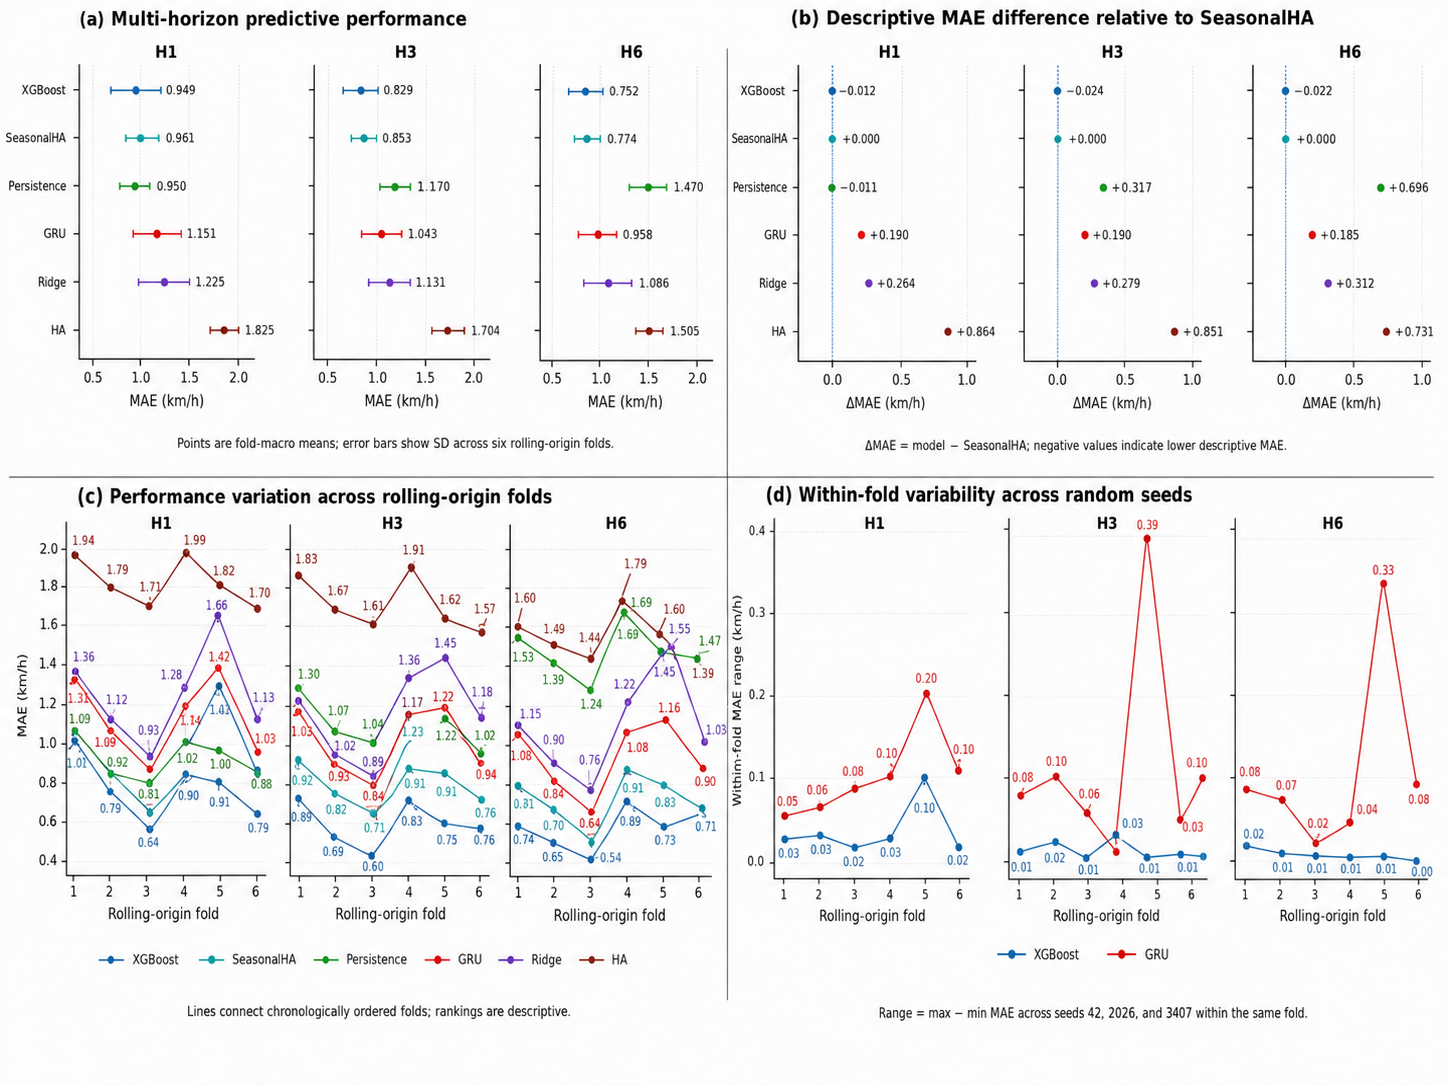
\includegraphics[width=0.97\textwidth]{Fig4.png}
    \caption{Multi-horizon forecasting performance and stability. Panels show fold-macro MAE, differences from SeasonalHA, fold-level MAE trajectories, and within-fold seed ranges for XGBoost and GRU. Rankings and differences are descriptive}
    \label{fig:performance_stability}

    \figurenote{Fold-macro summaries use the six retrospective rolling-origin folds, while the stochastic ranges in panel (d) are computed from seeds 42, 2026, and 3407. The panels are descriptive; inferential uncertainty is evaluated separately from these rankings.}
\end{figure}


Absolute errors are compared primarily within a horizon because H1, H3, and H6 average future windows of different lengths. The lower numerical MAE at H6 should not be read as evidence that six-hour forecasting is intrinsically easier; averaging over a longer window suppresses some short-term variation. Appendix~\ref{app:sensitivity} reports RMSE, sMAPE, and Bias as secondary checks. Their broad pattern is consistent with the MAE results, although individual rankings can differ by metric.

The fold-level inference does not establish the descriptive ordering as a stable difference. For XGBoost relative to SeasonalHA, mean $\Delta$MAE was $-0.0117$, $-0.0235$, and $-0.0222$~km~h$^{-1}$ at H1, H3, and H6. The corresponding 95\% unadjusted paired-bootstrap intervals were $[-0.1574,0.1825]$, $[-0.1210,0.0800]$, and $[-0.0837,0.0397]$, and Holm-adjusted p-values were 0.5625, 0.8438, and 1.000. Every interval crossed zero; none of the 15 prespecified comparisons was significant after Holm correction.

The supplementary day$\times$spatial-block estimates for XGBoost minus SeasonalHA were $+0.068$, $+0.025$, and $+0.023$~km~h$^{-1}$ at H1/H3/H6, with 95\% intervals of $[-0.151,0.376]$, $[-0.112,0.189]$, and $[-0.094,0.211]$. These intervals also include zero. Their signs differ from the fold-macro means because the two summaries weight temporal and spatial dependence differently, not because the underlying predictions differ.

\subsection{Cross-fold and random-seed stability}
\label{subsec:stability}

The model with the lowest overall mean was not the lowest-error model in every test period. Figure~\ref{fig:performance_stability}(c) shows XGBoost leading in four of six H1 folds and three of six folds at both H3 and H6; SeasonalHA led in the remaining folds. The H1 result for Fold~5 is a clear reversal: XGBoost recorded approximately 1.338~km~h$^{-1}$ and SeasonalHA 0.909~km~h$^{-1}$. Similar crossings at H3 and H6 indicate that the fold-macro mean alone does not describe temporal stability.

For XGBoost, variation across test periods was larger than variation across the three random seeds. Figure~\ref{fig:performance_stability}(d) measures within-fold stochastic variation by the MAE range across seeds 42, 2026, and 3407. Averaged over the 18 fold--horizon units, the range was 0.0193~km~h$^{-1}$ for XGBoost and 0.1038~km~h$^{-1}$ for GRU. The largest ranges were 0.0974~km~h$^{-1}$ for XGBoost at Fold~5--H1 and 0.3873~km~h$^{-1}$ for GRU at Fold~5--H3. Within this dataset and seed set, XGBoost is less seed-sensitive than GRU; the comparison is not generalized beyond the frozen training protocol.

\subsection{Reliability-conditioned forecasting performance}
\label{subsec:reliability-results}

The overall ranking changes when forecasts are separated by the reliability of their input history. Figure~\ref{fig:reliability_boundaries}(c) forms horizon-specific, error-blind quartiles from the pre-origin history-coverage ratio. At H1, the lowest-coverage quartile Q1 gives a fold-macro MAE of 1.109~km~h$^{-1}$ for XGBoost and 0.889~km~h$^{-1}$ for SeasonalHA. In Q4, the highest-coverage quartile, the ordering reverses to 0.774 and 0.886~km~h$^{-1}$, respectively. At H1, the nonlinear model's relative advantage changes with the information available before prediction.

H3 and H6 do not follow a simple monotonic pattern. At H3, XGBoost/SeasonalHA MAEs from Q1 to Q4 were approximately 0.893/0.794, 0.832/0.865, 0.795/0.876, and 0.684/0.799~km~h$^{-1}$; at H6 they were approximately 0.739/0.746, 0.791/0.836, 0.769/0.836, and 0.588/0.636~km~h$^{-1}$. The local crossings in the intermediate quartiles rule out a simple causal interpretation of coverage and do not define an optimal switching threshold. This non-monotonicity also shows why one global model ranking is insufficient for reliability-varying histories.

Figure~\ref{fig:reliability_boundaries}(a--b) shows that MAE and sample support also vary by node and fold, so high error should be read together with the number of valid forecast cases. Panel (d) adds the upper tail of the node-level error distribution. Across the formal node sequence, mean node-level median absolute error is approximately 0.30, 0.32, and 0.38~km~h$^{-1}$ at H1, H3, and H6; mean node-level P90 (90th-percentile) absolute error is approximately 1.97, 2.99, and 1.98~km~h$^{-1}$. Maximum P90 values reach approximately 4.75, 5.75, and 4.75~km~h$^{-1}$. The spatial audit does not provide a verified cumulative road-distance coordinate for every node, so the ordered node index in panel (d) cannot be used to label a persistent high-risk physical road segment.

\begin{figure}[!htbp]
    \centering
    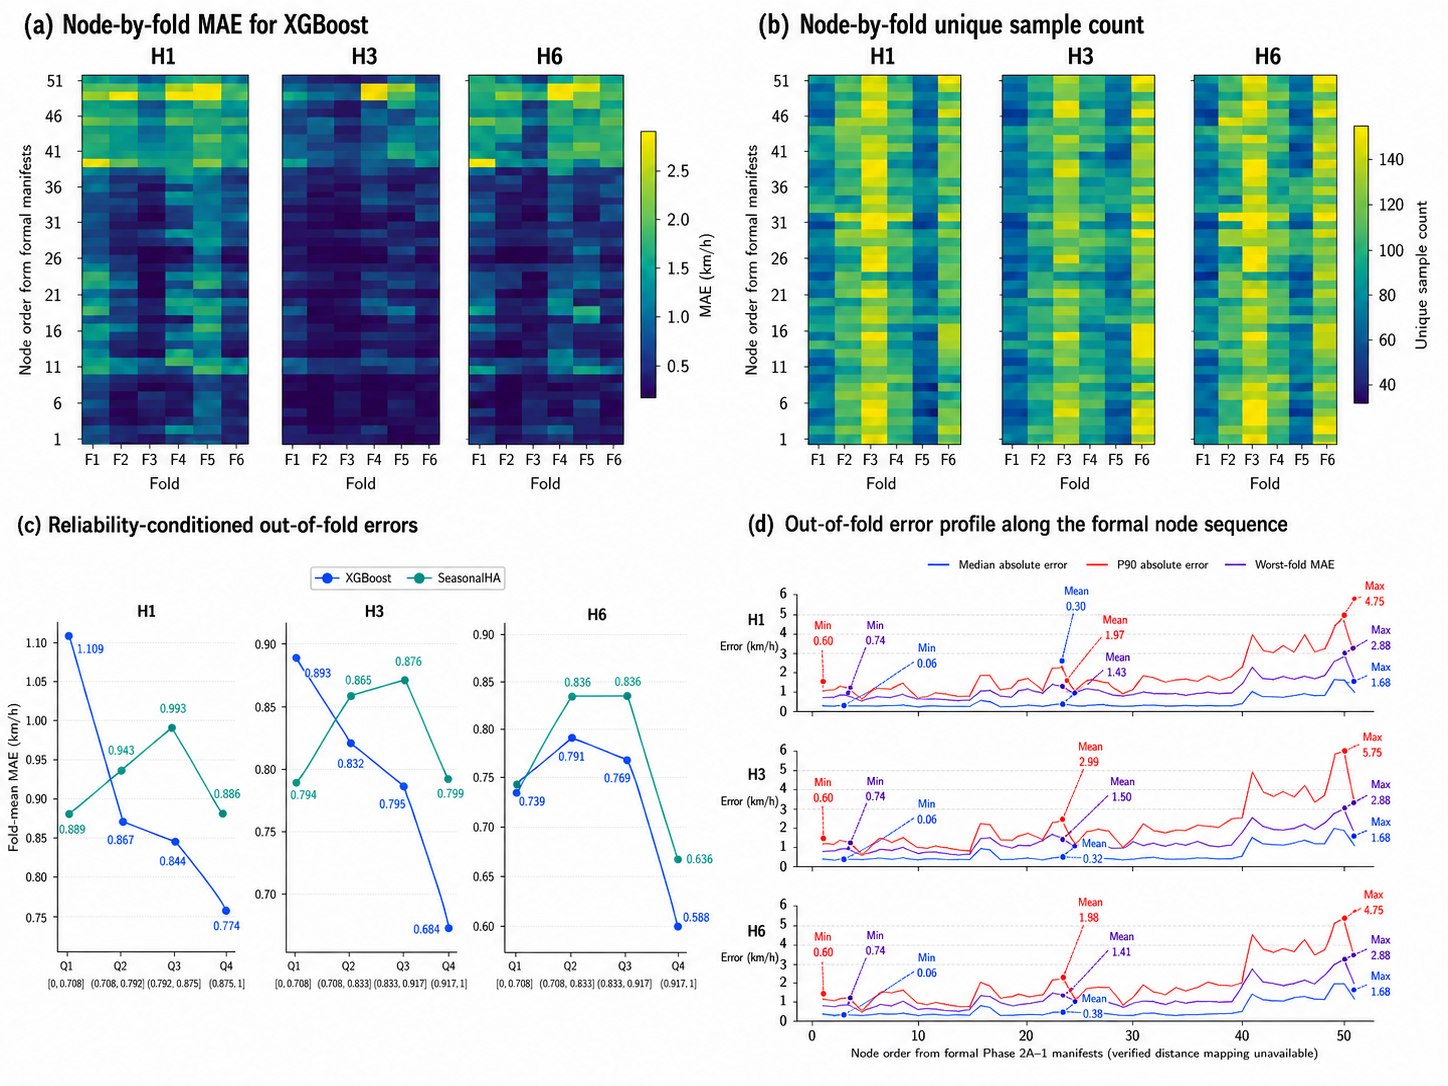
\includegraphics[width=0.97\textwidth]{Fig5.png}
    \caption{Reliability-conditioned and node-level error patterns. Panels summarize XGBoost node-by-fold MAE and support, XGBoost versus SeasonalHA across pre-origin coverage quartiles, and absolute-error profiles along the formal node sequence. Results are descriptive}
    \label{fig:reliability_boundaries}

    \figurenote{Coverage quartiles are defined from pre-origin history coverage without using forecast errors, and node-level error should be interpreted together with the corresponding sample support. The node sequence is an ordered manifest index rather than a verified cumulative road-distance axis, so the figure does not identify permanent high-risk road segments.}
\end{figure}

Figure~\ref{fig:statistical_boundaries} places the primary fold-level and supplementary clustered estimates on the same $\Delta$MAE scale.

\begin{figure}[!htbp]
    \centering
    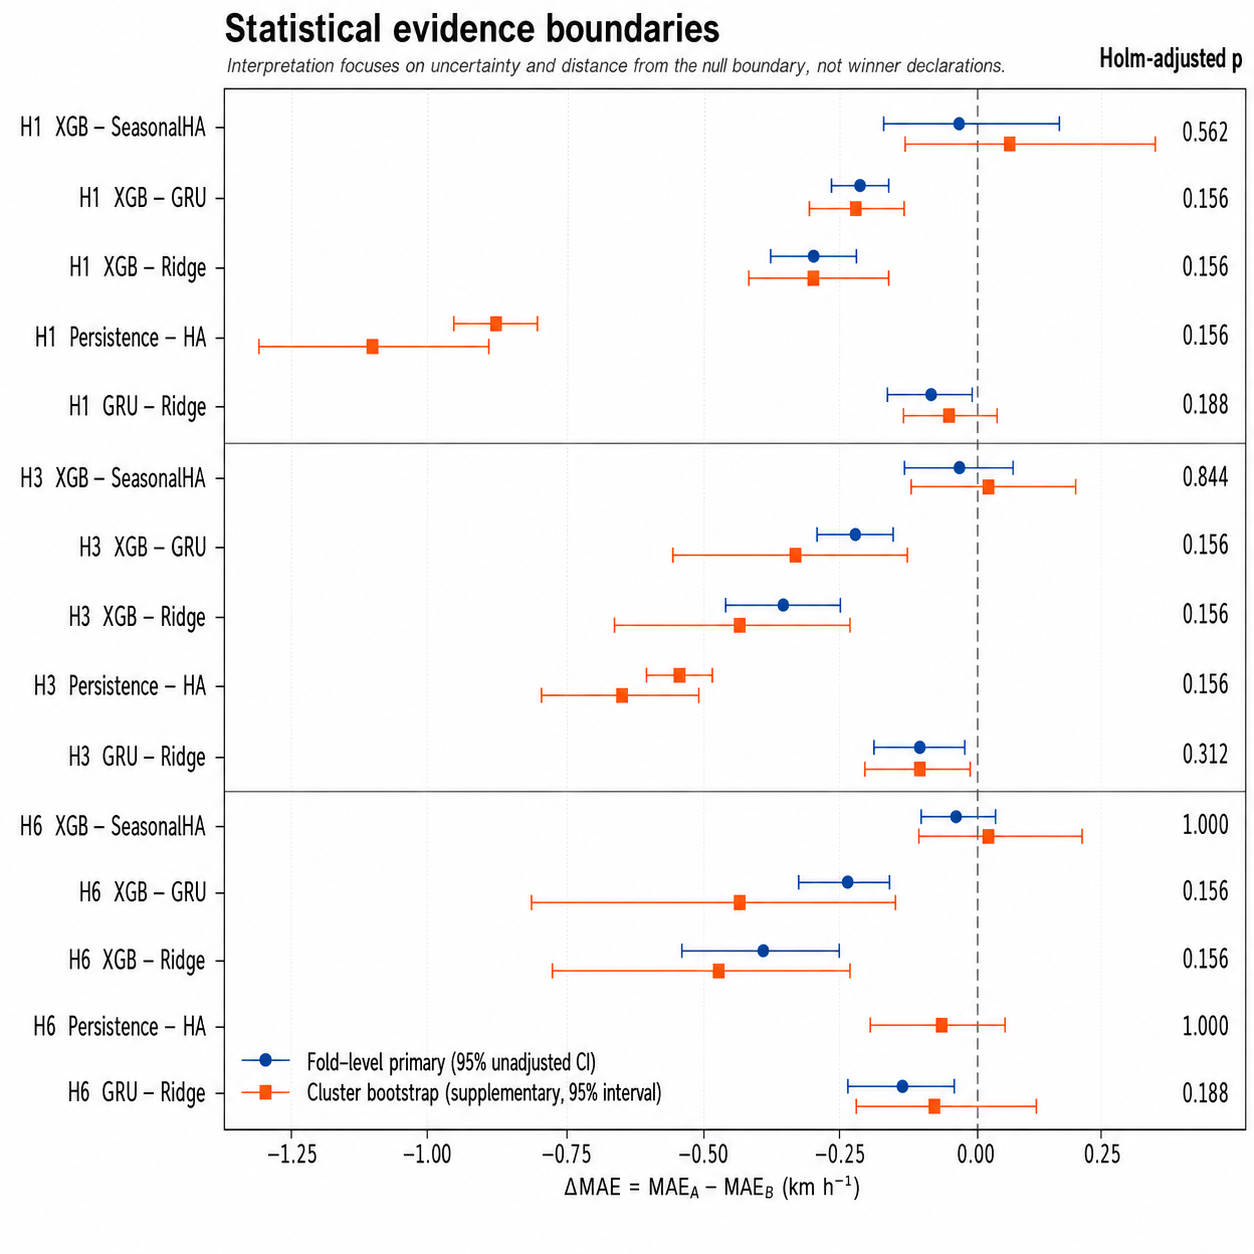
\includegraphics[width=0.88\textwidth]{Fig6.png}
    \caption{Uncertainty for the 15 prespecified paired comparisons. Negative $\Delta$MAE favors model A. The figure contrasts fold-level effects with supplementary day$\times$spatial-block bootstrap estimates and reports Holm-adjusted p-values}
    \label{fig:statistical_boundaries}

    \figurenote{Negative $\Delta$MAE indicates lower MAE for model A under the paired definition in Eq.~\eqref{eq:paired_delta}. Primary fold-level estimates and supplementary day$\times$spatial-block bootstrap estimates are shown together; none of the 15 Holm-adjusted Wilcoxon comparisons is statistically significant. Holm-adjusted p-values are rounded to three decimals in the figure, while the exact values for XGBoost--SeasonalHA are reported to four decimals in the text.}
\end{figure}


Model choice in this experiment depends on both horizon and history reliability. Persistence remains a useful H1 reference but loses value at H3 and H6. SeasonalHA stays competitive across horizons and is particularly strong in some lower-coverage conditions. XGBoost has the lowest descriptive mean error and its clearest H1 advantage occurs in the high-coverage group, yet the average gap from SeasonalHA is small compared with the variation across folds. In an operational pipeline, data eligibility should be checked before model selection; additional model complexity should not be used to compensate for an unreliable history. Cases that fail the history or target requirements are better flagged, assigned lower confidence, or rejected.

\subsection{Threats to validity}
\label{subsec:validity}

The findings are specific to the spatial and temporal scope of the experiment. The study covers one approximately 130-km Pan Borneo Highway corridor, 51 virtual nodes, and roughly three months of observations. Six rolling-origin test periods provide repeated out-of-time evidence, but they do not represent year-round seasonality, rare disruptions, or the full range of corridor traffic regimes. Relative model rankings and reliability patterns require confirmation on longer records and additional corridors.

The target itself imposes a second limitation. Forecast errors are calculated against provider-reported FCD speed, not against an independent measurement from loops, radar, or synchronized global navigation satellite system (GNSS) data. The experiment evaluates the temporal predictability of the commercial traffic-state product and does not validate the absolute accuracy of the provider's upstream speed estimates. Sampling, map matching, aggregation, and other provider-side processing remain outside the study's direct control.

The evaluation is retrospective rather than independently blinded. The terminal test period had been seen during earlier historical development, and the primary inferential sample contains only six paired folds. Statistical power is limited for small effects, which is reflected in the wide fold-level intervals. To avoid the opposite problem of pseudoreplication, the 92,147 test rows are not treated as independent inferential units.

Model and feature scope are also deliberately limited. The comparison uses six model types and a 24-h history without full network topology or rich exogenous inputs such as weather, incidents, and construction. The GRU result means only that recurrent sequence complexity did not produce a stable gain under this data scale and frozen training protocol; it is not evidence against deep traffic-forecasting methods as a class. The confidence threshold, 2-of-4 hourly rule, and H6 5-of-6 target rule should likewise be read as fixed engineering choices for this experiment rather than universally optimal settings.

A complete deployment-cost analysis is outside the present experiment. The archived environment records the principal workstation and software stack but not every final package microversion, energy measurement, or inference-cost component. Practical model selection would also have to account for retraining frequency, latency, maintenance, and computational resources.

A stronger validation design would prospectively lock the test period, add independent reference-speed measurements, extend the observation window, and repeat the protocol on other road classes, corridors, and FCD providers. Exogenous variables should be tested under the same common-manifest and causal-preprocessing constraints. Measuring training and inference resources would also allow the small accuracy differences reported here to be judged against deployment cost rather than error alone.
% ======================================================================
% 6 CONCLUSION
% ======================================================================

\section{Conclusion}
\label{sec:conclusion}

GATE-FCD was developed to make multi-horizon forecasting from sparse commercial FCD auditable before model rankings are interpreted. The framework reconstructs planned node--time combinations, separates missing from quality-ineligible records, builds causal 24-h histories, freezes common forecast samples, and checks the resulting predictions against leakage and consistency rules. The formal experiment produced 18 fold--horizon manifests and 180 completed model runs. All 20 full-sample audit assertions passed, with no detected future-information violation, target-recomputation mismatch, or cross-split target-window violation.

On these common samples, XGBoost had the lowest descriptive fold-macro MAE at H1, H3, and H6: 0.949, 0.829, and 0.752~km~h$^{-1}$. SeasonalHA was close at 0.961, 0.853, and 0.774~km~h$^{-1}$. Persistence was competitive at H1 but deteriorated at H3 and H6, while GRU and Ridge did not provide a stable gain that matched their additional modeling complexity under the present data scale and protocol. Because each horizon is a different future-window mean, these error magnitudes are interpreted within horizon rather than as evidence that the longer task is easier.

The descriptive XGBoost ranking was not statistically stable. Its mean MAE differences from SeasonalHA were only $-0.0117$, $-0.0235$, and $-0.0222$~km~h$^{-1}$; all three fold-level intervals crossed zero, and none of the 15 prespecified comparisons was significant after Holm correction. Rankings also reversed across test folds and history-coverage strata. At H1, SeasonalHA was better in the lowest-coverage quartile, whereas XGBoost was better in the highest-coverage quartile. No single model can be treated as the preferred choice across all horizons and reliability states.

These conclusions remain bounded by one corridor, one commercial FCD source, an approximately three-month record, provider-reported speed targets, and retrospective rolling-origin evaluation. Prospective testing, independent reference speeds, longer and cross-corridor datasets, additional providers and exogenous variables, and measured deployment costs are needed before broader generalization. GATE-FCD places data eligibility before model choice: a forecast case should first satisfy the observation, history, target, and temporal-causality requirements; only then should additional model complexity be judged against the required horizon and reliability condition.
% ======================================================================
% APPENDICES
% ======================================================================

\appendix

\section{Detailed eligibility and audit protocol}
\label{app:audit}

The formal data contract is fixed before model evaluation. Raw records are mapped to the complete 15-min node--time grid, screened using the frozen record-level criteria, deduplicated by arithmetic mean within identical node--quarter-hour keys, and aggregated to hourly speed under the 2-of-4 rule. A 24-row history $\{t_0-23,\ldots,t_0\}$ is then constructed for each candidate origin using causal forward fill followed, when necessary, by fold-training node-median and corridor-median fallback. Targets begin at $t_0+1$ and use no imputation. H1 requires 1/1 observed future hour, H3 requires 3/3, and the primary H6 definition requires at least 5/6.

The final manifest audit applied the following 20 assertions to 1,053,618 manifest records; every assertion passed with zero violations:
\begin{enumerate}
    \item sample identifiers are unique within the audited manifest structure;
    \item each model history contains exactly 24 hourly rows;
    \item history timestamps are strictly increasing;
    \item every history timestamp is at or before its forecast origin;
    \item every target timestamp is strictly after its forecast origin;
    \item the complete target window remains inside the assigned split;
    \item target values are never imputed;
    \item input history and target windows do not overlap;
    \item node identity is consistent across history, origin, and target;
    \item targets can be recomputed from the recorded source row identifiers;
    \item H1 requires 1 of 1 observed future hour;
    \item H3 requires 3 of 3 observed future hours;
    \item H6 requires at least 5 of 6 observed future hours;
    \item scaler parameters are fitted from fold-training data only;
    \item node and corridor fallback medians are fitted from fold-training data only;
    \item any regime threshold used by the pipeline is training-only or not used in the formal benchmark;
    \item backward filling is absent;
    \item centered rolling statistics are absent;
    \item future-data merges are absent; and
    \item all compared models use the same common sample manifest within each fold and horizon.
\end{enumerate}

The audit also verifies one-to-one matching between predictions and manifest rows, prediction-file and manifest hashes, the 180-run registry, and the frozen configuration lineage. These checks support internal reproducibility but do not convert the retrospective design into an independent blind test.

\section{Model hyperparameters and implementation details}
\label{app:hyperparameters}

Table~\ref{tab:appendix_hyperparameters} consolidates the frozen model settings used in the formal comparison. The same feature and target definitions are used across models; only the input representation and predictor differ.

\begin{table}[!htbp]
\centering
\caption{Frozen model and training settings used in the formal experiment.}
\label{tab:appendix_hyperparameters}
\footnotesize
\begin{tabularx}{\textwidth}{|>{\raggedright\arraybackslash}p{0.16\textwidth}|>{\raggedright\arraybackslash}X|}
\hline
\textbf{Component} & \textbf{Frozen setting} \\
\hline
HA & Mean of eligible fold--horizon training targets. \\ 
\hline
SeasonalHA & Mean of the frozen seasonally matched training reference set. \\ 
\hline
Persistence & Causally filled speed at forecast origin $t_0$. \\ 
\hline
Ridge & 315-dimensional tabular input; L2 penalty $\alpha=1.0$; deterministic. \\ 
\hline
XGBoost & 315-dimensional tabular input; 500 trees; maximum depth 8; learning rate 0.05; subsample 0.8; column subsample 0.8; objective \texttt{reg:squarederror}; \texttt{tree\_method=hist}; 10 CPU jobs; seeds 42, 2026, 3407. \\ 
\hline
GRU & $24\times13$ input; one GRU layer; hidden size 64; dropout 0.0; batch 256; learning rate $10^{-3}$; weight decay $10^{-4}$; maximum 30 epochs; patience 5; \texttt{minimum\_delta=0.0}; gradient clipping norm 1.0; seeds 42, 2026, 3407. \\ 
\hline
Stochastic aggregation & Average the three seed-level predictions for each sample before calculation of the primary metrics. \\ 
\hline
Input filling & Node-wise causal forward fill; if unavailable, fold-training node median, then fold-training corridor median. \\ 
\hline
Feature scaling & Each of the 13 sequence features standardized using the fold-training mean and population SD; validation and test use frozen training parameters. \\ 
\hline
Sequence input & 24 hourly rows $\times$ 13 standardized features. \\ 
\hline
Tabular input & Flattened 312 sequence values plus node order, latitude, and longitude = 315 dimensions. \\
\hline
\end{tabularx}
\end{table}


The formal campaign was run on a 64-bit Windows workstation with CPython~3.10 and an NVIDIA RTX A3000 Laptop GPU for the CUDA-enabled PyTorch workload. NumPy, pandas, PyArrow, scikit-learn, XGBoost, PyTorch, and SciPy formed the principal analysis stack. A complete final microversion and CUDA-version snapshot was not preserved in the archived environment record; no unverified microversions are reported here. The public repository instead preserves frozen configuration files, code and result revisions, common-manifest hashes, registered predictions, and audit outputs.

\section{Supplementary metrics and sensitivity analyses}
\label{app:sensitivity}

Table~\ref{tab:secondary_metrics} reports the six-fold means of RMSE, sMAPE, and Bias. These metrics are secondary to MAE but provide checks on large errors, relative error scale, and systematic signed error. The broad ordering is consistent with the primary analysis: XGBoost and SeasonalHA remain the leading pair at H3 and H6, while Persistence deteriorates substantially with horizon.

\begin{table}[!htbp]
\centering
\caption{Secondary fold-macro performance metrics. RMSE is in km~h$^{-1}$; sMAPE is in percent; Bias is in km~h$^{-1}$.}
\label{tab:secondary_metrics}
\footnotesize
\begin{tabular}{|l|l|r|r|r|}
\hline
\textbf{Horizon} & \textbf{Model} & \textbf{RMSE} & \textbf{sMAPE} & \textbf{Bias} \\
\hline
H1 & XGBoost     & 2.138 & 1.305 & -0.175 \\ 
\hline
H1 & SeasonalHA  & 2.399 & 1.379 & -0.026 \\ 
\hline
H1 & Persistence & 3.007 & 1.450 &  0.004 \\ 
\hline
H1 & GRU         & 2.333 & 1.577 &  0.124 \\ 
\hline
H1 & Ridge       & 2.455 & 1.672 & -0.141 \\ 
\hline
H1 & HA          & 3.738 & 2.818 & -0.039 \\
\hline
H3 & XGBoost     & 1.787 & 1.172 & -0.005 \\ 
\hline
H3 & SeasonalHA  & 1.793 & 1.209 & -0.002 \\ 
\hline
H3 & Persistence & 3.143 & 1.810 &  0.106 \\ 
\hline
H3 & GRU         & 1.852 & 1.417 &  0.089 \\ 
\hline
H3 & Ridge       & 2.021 & 1.551 & -0.046 \\ 
\hline
H3 & HA          & 3.300 & 2.644 &  0.003 \\
\hline
H6 & XGBoost     & 1.396 & 1.046 & -0.027 \\ 
\hline
H6 & SeasonalHA  & 1.467 & 1.089 & -0.004 \\ 
\hline
H6 & Persistence & 3.664 & 2.296 &  0.194 \\ 
\hline
H6 & GRU         & 1.641 & 1.307 &  0.067 \\ 
\hline
H6 & Ridge       & 1.821 & 1.476 & -0.091 \\ 
\hline
H6 & HA          & 2.874 & 2.341 &  0.009 \\
\hline
\end{tabular}
\end{table}


The supplementary day$\times$spatial-block bootstrap used 10,000 replicates, 41 test days, and five spatial blocks. For XGBoost minus SeasonalHA, the estimates were $+0.068$, $+0.025$, and $+0.023$~km~h$^{-1}$ at H1, H3, and H6, with 95\% intervals $[-0.151,0.376]$, $[-0.112,0.189]$, and $[-0.094,0.211]$. All intervals include zero. Their signs differ from the fold-macro means because the cluster estimator applies a different weighting and dependence structure.

A stricter H6 6-of-6 observed-hour requirement is retained as a prespecified sensitivity definition, whereas the primary formal target uses at least 5 of 6 observed hours. The main-text results and model rankings in this paper are based on the primary 5-of-6 contract and are not silently replaced by the stricter sensitivity rule. As an additional evidence-boundary diagnostic, the archived analysis notes that excluding Fold~6 changes the descriptive leader to SeasonalHA at H1 and H3 while XGBoost remains the descriptive leader at H6. This diagnostic is not treated as an alternative primary analysis; it reinforces the need to report the study as retrospective rather than independently blinded.

% ======================================================================
% BACK MATTER
% ======================================================================

\backmatter

\subsection*{Acknowledgments}

The authors thank the Faculty of Built Environment and Surveying, Universiti Teknologi Malaysia, for providing laboratory support. The authors also acknowledge the planning background information related to corridor operations in Sarawak, Malaysia, which helped clarify the practical context of this study. No individual or institution influenced the study design, data analysis, interpretation of the results, or conclusions of the manuscript.

\subsection*{Statements and Declarations}

\textbf{Funding.}

This research received no specific grant from any funding agency in the public, commercial, or not-for-profit sectors.

\textbf{Competing interests.}

The authors declare no competing interests.

\textbf{Author contributions.}

Wenjie Sun: Conceptualization, methodology, software, formal analysis, investigation, data curation, visualization, validation, and writing--original draft. Safizahanin binti Mokhtar: Conceptualization, methodology, supervision, project administration, validation, and writing--review and editing. Gabriel Ling Hoh Teck: Methodological review, validation, interpretation of results, and writing--review and editing. Ruiqing Li: Code and software review, literature review, model-method review, validation, and writing--review and editing. Lvmin Liu: Validation, interpretation of results, and writing--review and editing. All authors reviewed and approved the manuscript. 

\textbf{Ethics approval and consent to participate.}

Not applicable.

\textbf{Consent for publication.}

Not applicable.

\textbf{Data availability.}

The floating car data used in this study were obtained through the TomTom Traffic API. Raw provider data and sample-level records are not publicly redistributed because of provider licensing restrictions. Publicly shareable code, frozen configurations, aggregated results, and audit materials are provided through the project repository.

\textbf{Code availability.}

Public code, frozen configurations, aggregated results, and audit materials are available at
\url{https://github.com/tasadapullo-svg/FCD-for-Multi-Horizon-Highway-Speed-Forecasting_20260730}.

% ======================================================================
% REFERENCES
% ======================================================================

\bibliography{references}

\end{document}
